%% 
%% Author's note:
%% This was a template package which contains a lot of comments and code that were not written by me.
%%


%% Follow comments to support use.

%%%%%%%%%%%%%%%%%%%%%%%%%%%%%%%%%%%%%%%%%%%%%%%%%%%%%%%%%
%% STEP 1: Choose options for MSc / BSc / seminar layout and your bibliographic style
%%%%%%%%%%%%%%%%%%%%%%%%%%%%%%%%%%%%%%%%%%%%%%%%%%%%%%%%%

%%  Language: 
%%      finnish, swedish, or english
%%  Pagination (use twoside by default)  
%%      oneside or twoside,
%%  Study programme / kind of report
%%      csm  = Master's thesis in Computer Science Master's Programme;
%%      tkt = Bachelor's thesis in Computer Science Bachelor's Programme;
%%      seminar = seminar report
%%  For Master's thesis choose your line or track:
%%      (30 cr thesis, 2020 onwards, Master's Programme in Computer Science = csm)
%%      software-track-2020 = Software study track
%%      algorithms-track-2020 = Algorithms study track
%%      networking-track-2020 = Networking study track

\documentclass[english,twoside,censored,tkt]{HYthesisML} 


%% TODO: Check which is better (openright or openany).
% If wanted, open new chapters only at right page.
% By default, "openany".
%\PassOptionsToClass{openright,twoside,a4paper}{report}
\PassOptionsToClass{openany,twoside,a4paper}{report}

\usepackage{csquotes}
%%%%%%%%%%%%%%%%%%%%%%%%%%%%%%%%%%%%%%%%%%%%%%%%%%%%%%%%%
%% REFERENCES
%% Some notes on bibliography usage and options:
%% natbib -> you can use, e.g., \citep{} or \parencite{} for (Einstein, 1905); with APA \cite -> Einstein, 1905 without ()
%% maxcitenames=2 -> only 2 author names in text citations, if more -> et al. is used
%% maxbibnames=99 as no great need to suppress the biliography list in a thesis
%% for more information see biblatex package documentation, e.g., from https://ctan.org/pkg/biblatex 

%% Reference style: select one 
%% for APA = Harvard style = authoryear -> (Einstein, 1905) use:
\usepackage[style=authoryear,bibstyle=authoryear,backend=biber,natbib=true,maxnames=99,maxcitenames=2,uniquelist=minyear,giveninits=true,uniquename=mininit]{biblatex}
%% for numeric = Vancouver style -> [1] use:
%\usepackage[style=numeric,bibstyle=numeric,backend=biber,natbib=true,maxbibnames=99,giveninits=true,uniquename=init]{biblatex}
%% for alpahbetic -> [Ein05] use:
%\usepackage[style=alphabetic,bibstyle=alphabetic,backend=biber,natbib=true,maxbibnames=99,giveninits=true,uniquename=init]{biblatex}
%

\addbibresource{bibliography/bib_articles.bib}  
\addbibresource{bibliography/bib_books.bib}  
\addbibresource{bibliography/bib_inproceedings.bib} 
% in case you want the final delimiter between authors & -> (Einstein & Zweistein, 1905) 
% \renewcommand{\finalnamedelim}{ \& }
% List the authors in the Bibilipgraphy as Lastname F, Familyname G,
\DeclareNameAlias{sortname}{family-given}
% remove the punctuation between author names in Bibliography 
%\renewcommand{\revsdnamepunct}{ }

% Asked chat.openai.com: I'm using biblatex package, but it prints odd format volume.number in reference list, while this should be volume (number). How to fix this?
%Answer (shortened):
% Redefine the volume and number format
%\DeclareFieldFormat[article]{volume}{\mkbibbold{#1}}
%\DeclareFieldFormat[article]{number}{\mkbibparens{#1}}
% Please remove the boldface from the volume and number fields:
\DeclareFieldFormat[article]{volume}{#1}
\DeclareFieldFormat[article]{number}{\mkbibparens{#1}}
% Now this generated format volume.(number). How to remove the dot? (and so on with some adjustments):
\renewbibmacro*{volume+number+eid}{%
  \setunit{\addcomma\space}% 
  \printfield{volume}%
  %\setunit*{\addnbspace\addthinspace}% <-- Adjust spacing here
  \printfield{number}%
  \setunit{\addcomma\space}%
  \printfield{eid}}


%% Block of definitions for fonts and packages for picture management.
%% In some systems, the figure packages may not be happy together.
%% Choose the ones you need.

%\usepackage[utf8]{inputenc} % For UTF8 support, in some systems. Use UTF8 when saving your file.

\usepackage{lmodern}         % Font package, again in some systems.
\usepackage{textcomp}        % Package for special symbols
\usepackage[pdftex]{color, graphicx} % For pdf output and jpg/png graphics
\usepackage{epsfig}
\usepackage{subfigure}
\usepackage[pdftex, plainpages=false]{hyperref} % For hyperlinks and pdf metadata
\usepackage{fancyhdr}        % For nicer page headers
\usepackage{tikz}            % For making vector graphics (hard to learn but powerful)
%\usepackage{wrapfig}        % For nice text-wrapping figures (use at own discretion)
\usepackage{amsmath, amssymb} % For better math
\usepackage{comment}
\usepackage{booktabs}
\usepackage{array}
\usepackage{tabularx}

\singlespacing               %line spacing options; normally use single

\fussy
%\sloppy                      % sloppy and fussy commands can be used to avoid overlong text lines
% if you want to see which lines are too long or have too little stuff, comment out the following lines
% \overfullrule=1mm
% to see more info in the detailed log about under/overfull boxes...
% \showboxbreadth=50 
% \showboxdepth=50



%%%%%%%%%%%%%%%%%%%%%%%%%%%%%%%%%%%%%%%%%%%%%%%%%%%%%%%%%
%% STEP 2:
%%%%%%%%%%%%%%%%%%%%%%%%%%%%%%%%%%%%%%%%%%%%%%%%%%%%%%%%%
%% Set up personal information for the title page and the abstract form.
%% Replace parameters with your information.
\title{Generative AI in social engineering}


\author{Riku Talvisto}
\date{\today}

% Set supervisors, use the titles according to the thesis language
% in English Prof. or Dr., or in Finnish toht. or tri or FT, TkT, Ph.D. or in Swedish... 
\supervisors{Docent Lea Kutvonen}

\keywords{social engineering, artificial intelligence, AI, generative AI, cybersecurity, security, hacking, deepfake}
%\additionalinformation{\translate{\track}}
\additionalinformation{}

%% For seminar reports:
%%\additionalinformation{Name of the seminar}

%% Provide classification terms, to appear on the abstract page.
%% Replace the classification terms below with the ones that match your work.
%% ACM Digital library provides a taxonomy and a tool for classification
%% in computer science. Use 1-3 paths, and use right arrows between the
%% about three levels in the path; each path requires a new line.

%% TODO: Which are most suitable? Should I include one, 2 or 3? Should I include the document type (surveys and overviews) and is that correct?
%% TODO: Should any title be in bold or any in italics?
\classification{\protect{\ \\
\  Social and professional topics $\rightarrow$ Computing / technology policy  $\rightarrow$ Computer crime \\ $\rightarrow$ \textbf{Social engineering attacks} \\
%%\  Human-centered computing $\rightarrow$ Collaborative and social computing  $\rightarrow$ Collaborative and social computing theory, concepts and paradigms $\rightarrow$ Social engineering (social sciences) \\
\  Security and privacy $\rightarrow$ Intrusion/anomaly detection and malware mitigation \\ $\rightarrow$ \textbf{Social engineering attacks}
}}

%% If you want to quote someone special. You can comment this line out and there will be nothing on the document.
%\quoting{Bachelor's degrees make pretty good placemats if you get them laminated.}{Jeph Jacques}


%% TODO: Remember to make the final PDF a PDF/A compliant version for archival purposes!

%% OPTIONAL STEP: Set up properties and metadata for the pdf file that pdfLaTeX makes.
%% Your name, work title, and keywords are recommended.
\hypersetup{
    unicode=true,           % to show non-Latin characters in Acrobat’s bookmarks
    pdftoolbar=true,        % show Acrobat’s toolbar?
    pdfmenubar=true,        % show Acrobat’s menu?
    pdffitwindow=false,     % window fit to page when opened
    pdfstartview={FitH},    % fits the width of the page to the window
    pdftitle={},            % title
    pdfauthor={},           % author
    pdfsubject={},          % subject of the document
    pdfcreator={},          % creator of the document
    pdfproducer={pdfLaTeX}, % producer of the document
    pdfkeywords={something} {something else}, % list of keywords for
    pdfnewwindow=true,      % links in new window
    colorlinks=true,        % false: boxed links; true: colored links
    linkcolor=black,        % color of internal links
    citecolor=black,        % color of links to bibliography
    filecolor=magenta,      % color of file links
    urlcolor=cyan           % color of external links
}

%%-----------------------------------------------------------------------------------

\begin{document}

% Generate title page.
\maketitle

%%%%%%%%%%%%%%%%%%%%%%%%%%%%%%%%%%%%%%%%%%%%%%%%%%%%%%%%%
%% STEP 3:
%%%%%%%%%%%%%%%%%%%%%%%%%%%%%%%%%%%%%%%%%%%%%%%%%%%%%%%%%
%% Write your abstract in the separate file, to be positioned here.
%% You can make several abstract pages (if you want it in different languages),
%% in which case you should also define the language of the abstract,
%% as below.



% --------------------------------
% ABSTRACT (English)
% --------------------------------

\begin{otherlanguage}{english}
\begin{abstract}

\begin{comment}

Guides:
    - Max about 100-200 words
        - Some other theses have almost entirely covered the available area
    - If the abstract text is too full, is that demotivating to the reader?
    - Study material states that the abstract text is short, usually just one paragraph?
    - What has been studied
    - How it has been studied
    - What results have been observed
    - No references

TODO:
    [x] What is the research question
    [x] What is social engineering, quick definition?
    [x] How does modern AI augment SE attacks and countermeasures
    [x] What is analyzed in this thesis
    [x] Properly motivate the reader to read my thesis
    [ ] Explain that this is written in an easy-to-read manner?
    [x] What results have been observed

What to cover:
    - What is SE?
    - Modern AI
    - Attacks
        - Deepfake synthetic forgeries, videos, live voice morphing
        - Highly personalized phishing content (natural language processing), created with the help of chatbots like ChatGPT
    - AI augments both attacks and countermeasures
    - Countermeasures
        - User-oriented
            - User awareness & training programs
            - Simulated spear phishing campaigns using a variety of methods such as voice, text, live
            - Company policies
            - Company culture (erillinen company policies kohdasta)
        - Tech oriented
            - Real-time threat detection
    - Emerging challenges

From the student's material:
    - "Tiivistelmäteksti on lyhyt, yleensä yhden kappaleen mittainen (maksimissaan noin 100 sanaa) selvitys kirjoituksen tärkeimmästä sisällöstä: mitä on tutkittu, miten on tutkittu ja mitä tuloksia on saatu."

\end{comment}

Social engineering, a subdomain of cybersecurity, is the art and science of manipulating people into divulging confidential information or taking actions that may or may not be in their best interests. Traditionally, social engineering relied heavily on manual labor and human intuition, but with the advent of modern artificial intelligence (AI) technologies, cybercriminals are able to craft highly targeted and effective social engineering campaigns with novel, unexpected twists.

The research question this thesis seeks to address is how to protect end-users and organizations from social engineering attacks that are enhanced by generative AI technologies. To that end, this thesis explores the evolving landscape of AI in social engineering, focusing on attacks such as spear phishing aided by chatbots like ChatGPT and impersonation with hyper-realistic deepfake-generated forgeries. In contrast, the thesis also covers countermeasures against these attacks and evaluates their effectiveness based on relevant literature. Actualized incidents are briefly examined where appropriate.

The results indicate that AI-powered social engineering attacks are more convincing and successful than traditional attacks and that contemporary countermeasures against them are becoming increasingly ineffective. This highlights the urgent need for cybersecurity professionals to update their strategies and tools for cyber defense against the emerging threat of AI, as social engineering is a threat to every organization and every individual.



\end{abstract}
\end{otherlanguage}


% Place ToC
%\newpage
\mytableofcontents

\mainmatter

%%%%%%%%%%%%%%%%%%%%%%%%%%%%%%%%%%%%%%%%%%%%%%%%%%%%%%%%%
%% STEP 4: Write the thesis.
%%%%%%%%%%%%%%%%%%%%%%%%%%%%%%%%%%%%%%%%%%%%%%%%%%%%%%%%%
%% Your actual text starts here. You shouldn't mess with the code above the line except
%% to change the parameters. Removing the abstract and ToC commands will mess up stuff.
%%
%% Command \include{file} includes the file of name file.tex.
%% A new page will be created at every \include command, 
%% which makes it appropriate to use it for large entities such as book chapters. Cannot be nested.
%% It is useful for a big project, as changing one of the include targets 
%% won't force the regeneration of the outputs of all the rest.
%% Alternatively, \input is a more lower level macro 
%% which simply inputs the content of the given file like it was copy&pasted there manually.



\chapter*{Generatiivinen tekoäly käyttäjän manipulointihyökkäysten apuna\label{chapter:finnish}}
\begin{comment}

Tekoälyä hyödyntävä käyttäjän manipulointi
Teokälypohjainen käyttäjän manipulointi
Tekoälyavusteinen käyttäjän manipulointi

Pyydä Riinalta ym palautetta kieliopin tarkistuksessa! Opin samalla itse. Riinahan voi tarkistaa esim tätä .tex tiedostoa GitHubista? Tai PDF kumpi vaan hänelle parempi, mutta PDF:n kassa pitää muistaa aina päivittää se Overleafiin ja sitten GitHubiin.

Ohjeet:
    - 4 or 5 sivua
    - TOC ja Chapter 1 Introduction väliin

Kappaleet:
    - (ilman nimeä sisältää Introduction ja Definition kappaleet)
    - Hyökkäykset ja työkalut
    - Puolustuskeinot
    - Puolustuskeinojen arviointia
    - Yhteenveto
    - EI Overleaf kappalenumerointia? Kappale "0"?
    

\end{comment}


Käyttäjän manipuloinnilla (\textit{social engineering}) tarkoitetaan tietoturvan kontekstissa tietojärjestelmän loppukäyttäjään, eli ihmiseen, kohdistuvaa tietoturvahyökkäystä \citep{mitnickArtDeceptionControlling2003}. Sen sijaan että hyökkääjät etsisivät tietojärjestelmistä teknisiä haavoittuvuuksia, he kohdistavat hyökkäykset ihmiseen käyttäen hyväksi psykologisia menetelmiä \citep{wangDefiningSocialEngineering2020}.

Historiallisesti käyttäjän manipulointi on ollut riippuvainen ihmisen intuitiosta ja manuaalisesta työstä, mutta moderni tekoäly (\textit{artificial intelligence, AI}) on nyt muuttamassa koko kenttää uusiksi. Tekoälyn avulla hyökkääjät pystyvät luomaan uskottavia tietojenkalasteluviestejä (\textit{phishing}) sekä imitoimaan virallisia tahoja ja toimijoita realististen syväväärennösten (\textit{deepfake}), kuten kuvien, äänen ja jopa videoiden avulla.

Tässä kandidaatintutkielman suomenkielisessä lyhennelmässä käydään läpi tärkeimmät käyttäjän manipulointihyökkäykset sekä puolustuskeinot niihin.

\section*{Hyökkäykset ja työkalut}

Tunnetuin käyttäjän manipulointihyökkäys on tietojenkalastelu (\textit{phishing)}. Tietojenkalastelu on petollista toimintaa missä hyökkääjä esiintyy luotettavana tahona tavoitteenaan saada käyttäjältä luottamuksellisia tietoja kuten hänen salasanansa tai luottokorttinsa numeron. Kohdennettu tietojenkalastelu (\textit{spear phishing}) on kohdennettu tietylle käyttäjälle tai yritykselle, sisältäen jotain relevanttia tietoa kuten esimerkiksi käyttäjän nimen tai roolin yrityksessä.

OpenAI julkaisi vuonna 2022 ChatGPT:n joka mullisti tavan jolla ihmiset käyttävät tekoälyäpalveluita. Se keräsi yli 100 miljoonaa käyttäjää ensimmäisen kahden kuukauden aikana\footnote{https://explodingtopics.com/blog/chatgpt-users (luettu 2024-07-21)}. ChatGPT on ns. generatiivinen tekoäly (\textit{generative AI}) joka on koulutettu suurella määrällä tietoa ja joka pystyy tämän pohjalta luomaan uutta sisältöä, kuten tekstiä tai kuvia.

OpenAI ja muut tekoälypalveluita varmistavat yritykset ovat asettaneet käyttöehtoja, joiden puitteissa palvelun käyttö on sallittua. Rajoituksia käytölle on asetettu myös tekoälytoiminnallisuuksien sisälle. Hyökkääjät ovat kuitenkin onnistuneet valjastamaan ChatGPT:n kaltaiset suuret kielimallit (\textit{large language model}) omiin tarkoituksiinsa ohittamalla nämä rajoitukset.

ChatGPT ei esimerkiksi suoraan anna listaa sivustoista joilta voisi ladata laittomasti elokuvia, vaan sanoo että tämä toiminta on epäeettistä ja voi aiheuttaa käyttäjän tietokoneen saastumisen haittaohjelmilla (\textit{malware}). Tällaiset rajoitukset on pystynyt ohittamaan useilla eri keinoilla, esimerkiksi sanomalla että suojellakseen käyttäjää haittaohjelmilta ChatGPT:n pitäisi kertoa sivustoista joille käyttäjän ei tule mennä. Näin käyttäjä saa haluamansa tiedot käyttäen käänteistä psykologiaa.

Näin hyökkääjät ovat pystyneet käyttämään suurten kielimallien tekoälytyökaluja tietojenkalasteluviestien laatimisessa, mikä on huomattaavasti parantanut niiden uskottavuutta.

Syväväärennökset (\textit{deepfake}) ovat aidolta vaikuttavaa sisältöä kuten kuvia, ääntä tai videota, joka on luotu generatiivisen tekoälyn avulla. Syväväärennöksiä voidaan käyttää esimerkiksi opetusmateriaalina, mutta niitä voidaan käyttää myös petollisiin tarkoituksiin. Syväväärennöksiä on jo onnistuneesti käytetty käyttäjän manipulointihyökkäysten osana.

\section*{Puolustuskeinot}

Puolustautuminen tekoälyavusteisia käyttäjän manipulointihyökkäyksiä vastaan on pitkälti samankaltaista kuin tavallisiakin hyökkäyksiä vastaan, muutamilla muutoksilla. Puolustautumiskeinot voidaan jakaa karkeasti kahteen, ihmislähtöisiin ja tekniikkalähtöisiin.

Perinteinen tapa suojata käyttäjää tietojenkalasteluviesteitlä on ollut sääntöpohjainen suodattaminen (\textit{rule-based filtering}). Yksinkertaistettuna se vain tarkoittaa joukkoa loogisia sääntöjä joita seuraamalla voidaan päätellö onko viesti jollain todennäköisyydellä tietojenkalasteluviesti vai ei.

Sääntöpohjainen suodattaminen ei kuitenkaan toimi kovin hyvin tekoälyavusteista tietojenkalastelua vastaan. Tässä kohtaa tekoäly on valjastettu myös suojaamaan käyttäjää, eli siinä missä hyökkääjät käyttävät tekoälyä luodakseen kalasteluviestejä, puolustajat käyttävät sitä tunnistamaan näitä viestejä.

Historiallisesti ei ole ollut tarvetta tarkistaa saatujen kuvien tai videoiden aitoutta, mutta nyt syväväärennösten aikakautena käyttäjä ei voi luottaa näkemänsä materiaalin aitouteen vaan lisävarmistuksia on tehtävä. Yksi tapa on käyttää tekoälypohjaisia palveluita syväväärennösten tunnistamiseen, samaan tapaan kuin sähköpostiviestienkin tarkistaminen.

Käyttäjälähtöiset tavat ovat tyypillisesti olleet käyttäjien kouluttaminen, simuloidut käyttäjän manipulointihyökkäykset, yrityksen tietoturva- ja tietosuojaohjeistusten laatiminen ja käytön valvonta, sekä tietoturva- ja tietosuojatietoisen yrityskulttuurin rakentaminen.

Tekoälypohjainen käyttäjän manipulointi tuo joitain muutoksia käyttäjälähtöisille puolustuskeinoille. Ensinnäkin käyttäjät eivät enää voi luottaa siihen, että hyvinkään kirjoitettu viesti ei olisi tietojenkalasteluviesti. Toiseksi kaikki saatu materiaali, kuten kuvat, äänitiedostot ja videot, saattavat olla syväväärennöksiä, vaikka käyttäjä ei itse pystyisi huomaamaan niissä mitään epätavallista.

Koska tekoälyohjelmat pystyvät automaattisesti etsimään Internetistä tietoa joita voisi käyttää osana käyttäjän manipulointihyökkäyksiä, myöskään viestit joissa on maininta joistain käyttäjälle relevanteista, ehkä jopa henkilökohtaisista asioista, ei voida enää varmuudella sanoa olevan aitoja.

\section*{Puolustuskeinojen arviointia}

Tässä luvussa käydään arvointia puolustuskeinojen tehokkuudesta.

Tekoälyavusteisten hyökkäysten torjuminen pohjautuu hyvin paljon samoille tekniikoille jotka ovat jo käytössä: sisääntulevan viestinnän tarkistaminen, käyttäjien kouluttaminen, simuloidut hyökkäykset, yrityskulttuurin rakentaminen ja tietoturvaohjeistusten ylläito. Jokaiseen näihin kuitenkin on tehtävä muutoksia generatiivisen tekoälyn luoman uuden uhan vuoksi.


\section*{Yhteenveto}

Vaikuttaa siis siltä että voimme olettaa tekoälyjärjestelmien nopean kehittymisen jatkuvan, tietoturvauhkien kehittymisen niiden mukana, ja tarpeen jatkuvalle käyttäjien kouluttamiselle ja uusien puolustuskeinojen löytämiselle kasvavan.

[FILLER ROW]

[FILLER ROW]

[FILLER ROW]

[FILLER ROW]

[FILLER ROW]

[FILLER ROW]

[FILLER ROW]

[FILLER ROW]

[FILLER ROW]

[FILLER ROW]

[FILLER ROW]

[FILLER ROW]

[FILLER ROW]

[FILLER ROW]

[FILLER ROW]

[FILLER ROW]

[FILLER ROW]

[FILLER ROW]

[FILLER ROW]

[FILLER ROW]

[FILLER ROW]

[FILLER ROW]

[FILLER ROW]

[FILLER ROW]

[FILLER ROW]

[FILLER ROW]

[FILLER ROW]

[FILLER ROW]

[FILLER ROW]

[FILLER ROW]

[FILLER ROW]

[FILLER ROW]

[FILLER ROW]

[FILLER ROW]

[FILLER ROW]

[FILLER ROW]

[FILLER ROW]

[FILLER ROW]

[FILLER ROW]

[FILLER ROW]

[FILLER ROW]

[FILLER ROW]

[FILLER ROW]

[FILLER ROW]

[FILLER ROW]


%% Chapters




% --------------------------------
% INTRODUCTION
% --------------------------------


\chapter{Introduction\label{chapter:intro}}
\begin{comment}

Guides:
    - Find more things into this guides list
    - Page limit 1-2 pages
    - Context, who needs, what is needed, why is it a problem
    - Research question and research methodologies
    - Summary of results
    - What roles each section will have
    - No subsections

TODO:
    [ ] Who is this thesis for
    [ ] Why should you read my thesis
    [ ] What is the research question and how it is answered
    [ ] How is this thesis organized, what is covered and what is deliberaly not covered and in what chapters (outline)

What to cover:
    - Motivate the user to read my thesis!
    - What is cybersecurity and why it's of paramount importance
    - What is SE?
    - Modern AI
        - Large Language Models
        - Emergence of ChatGPT and the like
    - Attacks
        - Deepfake synthetic content, videos, live voice morphing
        - Highly personalized phishing content (natural language processing)
        - Automated OSINT gathering
    - AI augments both attacks and countermeasures
    - Countermeasures
        - User awareness & training programs
        - Company policy & company culture
        - Real-time threat detection
        - Vulnerability detection
    - Emerging challenges
    - Motives for cybercrimes
        - Hard(er) to detect?
        - "Easy" wins?
    - Evolution of SE tactics and their impact on organizations
    - Intro to AI and its applications in cybersecurity
    - Research ga in the literature regarding the intersection of SE and AI


Info from lecture materials:
    - Johdannon tarkoituksena on kertoa yleiskielisesti työn tavoite. Kerrotaan (kuten tiivistelmässäkin, mutta laveammin), mitä on tutkittu, miten on tutkittu ja mitä tuloksia on saatu. Jotta kysymyksenasettelu ja tulokset on lukijan helppo oikein tulkita on syytä aloittaa johdanto asettelemalla tutkimus asiayhteyteensä, esimerkiksi kertomalla aluksi, minkälaisessa yhteydessä tarkasteluun otettavat haasteet esiintyvät ja keiden on ratkaisuista tarkoitus hyötyä.

    - Johdannon pituus määräytyy suhteessa koko kirjoitelman pituuteen. Parisivuinen kirjoitus ei erikseen otsikoitua johdantoa kaipaa, sillä se itsessään on laajennettu tiivistelmä. Kymmensivuisen kirjoituksen johdanto voi olla vaikkapa sivun tai puolentoista mittainen. Pro gradu -tutkielman 50-70-sivuiseen kokonaisuuteen tuntuu 2-4-sivuinen johdanto kohtuulliselta.

    - Johdanto kertoo siis lyhyessä, yleistajuisessa muodossa koko kirjoitelman kysymyksenasettelun, juonen sekä tulokset ja johtopäätelmät. Tämän luettuaan lukija voi päätellä, haluaako syventyä asiaan tarkemmin lukemalla koko kirjoituksen.

\end{comment}

The widespread adoption of interconnected IT devices and services has transformed every aspect of human life, from personal communication to business operations, and this reliance seems to be ever-expanding. The digital revolution has created numerous opportunities but has also introduced significant vulnerabilities. Among these, social engineering poses a particularly grave threat to security and privacy.

Social engineering is the art and science of manipulating victims into divulging confidential information or performing actions that may or may not be in their best interests \citep{hadnagySocialEngineering2018}. Rather than looking for technical vulnerabilities, social engineering relies on human interaction and exploits weaknesses in human psychology \citep{wangDefiningSocialEngineering2020}.



%For illustration, famous case studies are also examined.

Historically, social engineering relied heavily on human intuition and manual effort to deceive targets \citep{mitnickArtDeceptionControlling2003}. With the advent of modern artificial intelligence (AI), the landscape of social engineering is undergoing a  significant transformation, augmenting the sophistication and effectiveness of current and emerging attack methods \citep{fakhouriAIDrivenSolutionsForSocialEngineeringAttacks2024}.

%Certain social engineering attacks that are of particular interest when it comes to AI were chosen for more in-depth analysis, such as phishing, vishing (voice phishing), automated intelligence gathering, and deepfake-generated content, while leaving other attacks with less focus, such as dumpster diving, shoulder surfing, and tailgating.

This thesis explores the intersection of AI and social engineering and how contemporary AI technologies enhance the execution and impact of these attacks, and discusses the necessary actions to counter such advanced attacks. Several social engineering attack vectors and tools particularly relevant to the modern threat of AI were selected for in-depth analysis: spear phishing with the help of chatbots like ChatGPT, impersonation through deepfake-generated images, audio, and video, and the automated gathering and processing of intelligence data.

%The thesis discusses countermeasures, emphasizing the need to enhance current cybersecurity training and awareness programs to address the modern AI threat. The primary focus is on the human aspect of social engineering, while the technical details of AI tools and techniques are beyond the scope of this thesis.

%Countermeasures that are especially covered include how current cybersecurity training and awareness programs need to be augmented for the modern threat of AI. The major focus of this thesis is in the human element of social engineering, and the technical details of AI tools and techniques are outside of this thesis's scope.

%Next, key ideas and concepts in the field of social engineering are examined before moving on to the anatomy of a typical social engineering attack so that the actual attacks can be discussed in their proper context, all of this before we can finally delve into the countermeasures against the discsused attacks.

Based on a literature review and analysis of occurred social engineering incidents, the results indicate that contemporary countermeasures against social engineering attacks are ill-equipped to deal with the sophistication of AI-powered threats \citep{fakhouriAIDrivenSolutionsForSocialEngineeringAttacks2024, blauthArtificialIntelligenceCrime2022}. Thus, the urgent need for cybersecurity professionals to update their tools and strategies is evident; however, AI can also play a valuable role in this area.





%
% ORGANIZED
%

The rest of the thesis is structured as follows: Chapter \ref{chapter:definition} introduces social engineering, generative AI, and other essential concepts for further analysis. Chapter \ref{chapter:attacks} examines relevant attack vectors and tools, including spear phishing and deepfake impersonation. Chapter \ref{chapter:countermeasures} then discusses both technological and human-oriented countermeasures against these attacks. The effectiveness and viability of these measures are then assessed in Chapter \ref{chapter:evaluation}. Lastly, Chapter \ref{chapter:conclusions} summarizes key findings and implications for the future of social engineering defense.




%Despite advancements in cybersecurity measures, social engineering remains a persistent threat. High-profile data breaches and corporate espionage incidents underscore the efficacy of social engineering techniques. Often, sophisticated firewalls, encryption algorithms and intrusion prevention systems (IPS) and intrusion detection systems (IDS) can be rendered useless by a cleverly worded email or an unsuspecting phone call. While it's often said that the most secure computer is one that is not plugged in, with social engineering an attacker could persuade someone to plug it in and turn it on.

%This study seeks to investigate the diverse aspects of social engineering, focusing on its techniques, effects, and prevention measures. Grasping the concept of social engineering is essential, not just for cybersecurity experts but also for people and organizations in every sector and at all employment levels. The increasing sophistication of social engineering attakcks coupled with the integration of artificial intelligence (AI) and technologies such as deepfakes (deep learning, fake) pose a growing risk that transcends traditional security frameworks. Because of this, extra attention is paid to how AI is and might contribute to the field of social engineering, both in terms of attacks and defenses.

%By dissecting real-world case studies and theoretical underpinnings, this thesis will provide a comprehensive overview of social engineering, contributing to the broader effort of mitigating its risks.

%Efficacy of social engineering training and awareness programs varies, with main challenges lying in user's interest and motivation towards the training and retention of learned data. Continued education, especially because social engineering is a constantly evolving field where the attackers never cease to improvise, is absolutely essential. Gamification, and users's inward motivation, go a long way in achievehing this.



%Usually when IT experts talk about an information system, they focus on the technical parts, the devices. But most, if not all, IT systems are useless without at least some interface with the people using it. Thus, especially from the social engineering standpoint, it's more beneficial to think of an information system as comprising the technology and its users. With this in mind, it becomes evident that the attack surface a hacker has is vast, and like water flowing down a river, the hacker often chooses the path of least resistance. Time and time again it has been proven that the easiest, most cost-effective way in is through the human factor of the IT system. Bolstering just one facet of this system is like fixing a leak or a potential leak only in some places, and not looking at the whole situation holistically. Security and privacy are a 360 degree, 24/7 thing.

%Currently, social engineering attacks are the biggest threat facing cybersecurity.


%This thesis is organized as follows. First, social engineering is defined and some history explained. Next, the different stages of a social engineering attack are examined. Then multiple common attack methods are discussed along with how modern AI powers them up. After that, AI-powered countermeasures are examined. The final chapter conclues this thesis.






% --------------------------------
% SOCIAL ENGINEERING & AI
% --------------------------------
    

\chapter{Social Engineering and AI\label{chapter:definition}}
\begin{comment}

Guides:
    - Page limit 1-2 pages
    - Context and terminology (käsitteet), challenges and measurement criteria, values, research question analysis
    - Second to last paragraph contains the research question (RQ) and the results

TODO:
    [ ] 

What to cover:
    - What is cybersecurity and why it's of paramount importance
    - What is social engineering
        - Brief history of social engineering
            - Phishing in 1996 via AOL
    - Attacks, classical social engineering attacks
        - Phishing, vishing, smishing
        - Tailgating
        - Baiting (not always considered SE)
        - Dumpster diving (not always considered SE)
    - Countermeasures, classical
        - User awareness & training programs
        - Company policy & company culture
        - Real-time threat detection
        - Vulnerability detection
    - Typical challenges
    - Motives for cybercrimes
        - Hard(er) to detect?
        - "Easy" wins?

Literature:
    - Defining Social Engineering in Cybersecurity

\end{comment}

This chapter gives an overview of what social engineering constitutes, provides brief historical context and describes some key terminology that is necessary for further analysis, including about AI. After this, Chapter \ref{chapter:attacks}  examines AI-powered attack methods and tools.

The term \textit{social engineering} dates back to 1842, when it was used to describe centralized planning in an attempt to manage the future development and behavior of a society \citep{hatfieldSocialEngineeringCybersecurity2018a}. Since then, its use has shifted to the field of cybersecurity through the phone phreaking phase (late 1950s to early 1970s) and through to the contemporary hacker culture \citep{wangDefiningSocialEngineering2020}.

As one of the earliest hackers and social engineers, the phreakers, used impersonation to call the Bell Telephone company in order to gain insider information about the telephone networks in order to carry out further attacks without the need for social manipulation \citep{hatfieldSocialEngineeringCybersecurity2018a}, modern hackers view social engineering not as something to be replaced but a key part of any hacker's toolkit, in fact perhaps the most important one \citep{mitnickArtDeceptionControlling2003}.

%Interconnected computers on a network are usually represented via a node structure. Business operations, from the perspective of social engineering attacks, can also be represented in this way, with the addition of other attack vectors into the map, such as employees, contractors, entryways, trash dumpsters and any and all other means an attacker could attack an organization. Thus the organization forms a system, with the computers and other network equipment forming only a part of the system, with at least one person always using it. Figure 3 represents such an attacker's view on an organization.

A strict consensus regarding the definition of a social engineering attack is lacking in the field  \citep{hatfieldSocialEngineeringCybersecurity2018a}. For the purposes of this thesis, social engineering is defined as "\textit{a type of attack wherein the attacker(s) exploit human vulnerabilities by means of social interaction to breach cybersecurity, with or without the use of technical means and technical vulnerabilities}" \citep{wangDefiningSocialEngineering2020}.

Some key concepts, namely open-source intelligence, pretexting, and generative AI, are explained next.









% --------------------------------
% Open-Source Intelligence
% --------------------------------
\section{Open-source intelligence}
\begin{comment}

    - OSINT, sometimes written as OS-INT?
    - Data from publicly available resources
        - Company website
        - Social networking sites
        - Sites like archive.org and Google archives
        - Observing people in real life
    - Does not include calling the company and asking for information or any other forms of engagement
    - How modern AI augments OSINT gathering is analyzed in the last chapter
        - Exploration of how AI tools and techniques used for the automation and enhancement of OSINT processes
    - Stress the importance of OSINT within SE
    - Ethical considerations when it comes to OSINT
    - Some case studies highlighting the use of OSINT in real-world social engineering incidents?
    - Countermeasures will also be covered later
        - Strategies for companies to mitigate the risks associated with OSINT-based attacks
        - Integration of AI algorithms for analyzing and extracting valuable insights from OSINT data
        - Impact of AI-powered intelligence gathering of SE attacks
        
\end{comment}

In social engineering, publicly available information is referred to as \textbf{open-source intelligence}. Like the name implies, it involves gathering of intelligence data from publicly locatable sources, such as from the target company's website, or from the social networking profiles of an individual or from other public records.

Various online tools exist for the purposes of gathering intelligence on an individual or an organization, the most famous of which in 2024 is perhaps Maltego. It offers automated forensic gathering and visualizes the found data, making it easier to identify patterns and connections.

Social engineering attacks typically begin with the gathering of open-source intelligence, which are subsequently used in conjunction with pretexting to attack an individual or an organization.










% --------------------------------
% Pretexting
% --------------------------------

\section{Pretexting}
\begin{comment}

    - General info about what is pretexting
    - Fabricated scenario that is plausible but fraudulent
    - Originally used by FBI
    - Impersonation
    - Discussion about how modern AI can aid with pretexting is in the final chapter
    - Role in the deception-based SE attacks
    - Common pretexting tactics will be covered later
    - How AI powers up pretexting will be discussed later
        - How AI tech can be utilized to create more sophisticated and convincing pretexts
        - Examples of successful pretexting attacks and their impacts
        - AI and automated pretexting attacks and their effectiveness
        - Analysis of pretexting evolving landscape with AI
    - Ethical considerations?
    - Countermeasures will be covered later also
        - How to identify and mitigate attempts
        - Recommendations for organiations to enhance their defenses against pretexting attacks
        
\end{comment}

Pretexting involves fabricating a story or a scenario, a \textbf{pretext}, that is plausible but fraudulent, to engage the target  with \citep{contehCybersecurityRisksVulnerabilities2016, fakhouriAIDrivenSolutionsForSocialEngineeringAttacks2024}. With this story, the attacker hopes to gain the victim's trust by appearing legitimate. This type of attack relies heavily on the gathered open-source intelligence in assisting with the creation of the story \citep{hadnagySocialEngineering2018}.

Pretexting uses psychological manipulation, trust and relationship-building, making it a potent tool for attackers \citep{mitnickArtDeceptionControlling2003}. The attacker, often assuming the likeness and character of a legitimate entity such as a trusted colleague, an IT service worker, a government official, or a 3rd party service provider, creates a believable narrative story tailored to the target victim's context.

%The success of pretexting is based on the attacker's ability to gather background OSINT and use it convincingly, making the pretext appear legitimate and aligned with the target victim's expectations or experiences \citep{mitnickArtDeceptionControlling2003}.














% --------------------------------
% Generative AI
% --------------------------------

\section{Generative AI}
\begin{comment}

Artificial Intelligence, Generative AI (ChatGPT, etc)

What to cover:
    - Mitä tekoäly oikeastaan edes on?
    - What is Generative AI
    - OpenAI releasing ChatGPT to the public in 2022
    - NLP Natural Language Processing
    
What to skip:
    - GPT:n historian (versiot 1, 2, 3, 3.5 jne) eli keskitytään vain GPT versioon 4 ja uudempiiin
    
\end{comment}

When AI is used to generate content, it is called \textbf{generative AI} \citep{goodfellowGenerativeAdversarialNetworks2020}. Unlike traditional AI, which follows programmed rules, generative AI utilizes machine learning to learns patterns from large training datasets to produce new outputs, such as text, images, audio and video \citep{fakhouriAIDrivenSolutionsForSocialEngineeringAttacks2024}.

A key example of generative AI is ChatGPT\footnote{https://openai.com/index/chatgpt (accessed 2024-08-19)}, a chatbot released by OpenAI in 2022. While far from being the first \citep{weizenbaumELIZA1996}, this chatbot revolutionized how people use and interact with AI systems, reaching over 100 million users in just two months\footnote{https://explodingtopics.com/blog/chatgpt-users (accessed 2024-08-11)}. Built on the GPT (Generative Pre-trained Transformer) architecture, ChatGPT is designed to understand and generate human-like text by predicting the next word in a sequence. It utilizes natural language processing (NLP), a domain at the intersection of human language and computation.

Another prominent form of generative AI is OpenAI's DALL-E project. It understands human written text and generates images based on the user's prompt.




% --------------------------------
% ATTACK VECTORS AND TOOLS
% --------------------------------

\chapter{Attack vectors and tools \label{chapter:attacks}}
\begin{comment}

Guides:
    - About 3-4 pages

TODO:
    [ ] 

What to cover:
    - Attacks
        - Deepfake generated synthetic media
            - Videos
            - Images
            - Audio
            - Real-time voice morphing

Sections:
    - Attack Vectors and Tools
        - Chatbots
        - Deepfake-generated media
        - Phishing & spear phishing

\end{comment}

This chapter reviews key social engineering attack vectors and tools relevant to the modern threat of generative AI. It first explores the misuse of chatbots like ChatGPT for malicious content generation. The discussion then covers deepfake-generated media that can be used for impersonation, concluding with how attackers could use all of this with spear phishing. After this, Chapter \ref{chapter:countermeasures} goes over the countermeasures against these attacks.













% --------------------------------
% Chatbots
% --------------------------------

\section{ChatGPT and other chatbots}

\begin{comment}

What to cover:
    - Mitä ovat chatbotit kuten ChatGPT
    - How Generative AI can be used by both cybersecurity professionals and threat actors
    - Circumventing ChatGPT's ethical restrictions with, for example prompt injections attacks or reverse psychology (with at least 1-2 examples)
    - How scholars and regular users have found ways to bypass ChatGPT's ethical restrictions??
    - Tekoälyn päivitys kun löydetään uusia tapoja ohittaa sen eettiset ohjeistukset ja kehittäjien asettamat rajoitukset
    - Pyydetään tekoälyä roolipelaamaan social engineering skenaarioita
    - Kielioppi ja kirjoitusvirheiden korjaus scam viesteissä
    
\end{comment}

Malicious actors can use generative AI  \textbf{chatbots} such as ChatGPT in their schemes, but due to the manufacturer's set limits, some workarounds may need to be used \citep{guptaFromChatGPTtoThreatGPT2023}. For instance, when asking ChatGPT to provide links to websites that provide pirated content such as movies results in the chatbot denying the request, stating that downloading pirated content is unethical and may also lead to the user's computer being infected with malware.

% ChatGPT reached 100 million users in 2 months https://explodingtopics.com/blog/chatgpt-users

However, regular users and scholars have found a number of ways to bypass ChatGPT's inherent ethic and behavioral guidelines, such as by using reverse psychology\footnote{https://incidentdatabase.ai/cite/420 (accessed 2024-07-15)}. In the above example, instead of directly asking for links to the pirate websites, the user can say that because he does not want his computer to be infected by malware, ChatGPT should provide links to sites the user should avoid visiting, thus causing ChatGPT to reveal the content the user originally wanted.












% --------------------------------
% Deepfake-generated content
% --------------------------------

\section{Impersonation with deepfakes}
\begin{comment}
Deepfake-generated content

What to cover:
    - What is a deepfake
    - Deepfakeja ei käsitely aiemmin? Generative AI kappaleessa?
    - Seuraava section kertoo tietojenkalastelusta ja sitoo chatbotit, automated intelligence gathering ja nää deepfaket yhteen kokonaisuudeksi

\end{comment}

\textbf{Deepfake}, a portmanteau of "deep learning", a type of machine learning, and "fake", is technology which uses artificial neural networks to create highly convincing fake media, either by altering existing content or creating them from scratch \citep{mirskyTheCreationAndDetectionOfDeepfakes2021}. When existing content is being altered, it's called reenactment or replacement, and when entirely new content is created, it's called synthesis. Deepfake content can be images, audio, and even full-resolution video. These hyper-realistic forgeries can depict a person saying or doing things that didn't actually happen, making it difficult for people and AI systems to discern what is real and what is fake \citep{blauthArtificialIntelligenceCrime2022}.

By utilizing deepfake-generated content, deepfakes, attackers can convincingly impersonate trusted individuals or organizations, enhancing the credibility and even the emotional impact of their deceptive strategies \citep{mirskyTheCreationAndDetectionOfDeepfakes2021}. Complete facial reenactment (pose, gaze, blinking, mouth etc) was achieved with only one minute of training video, suggesting that if a malicious actor wants to reenact an individual, they don't need to gather a lot of video material for this. If video material is not available, attackers can resort to filming the target person exiting the company's premises.

In 2024, deepfake technology was used in a video conference\footnote{https://incidentdatabase.ai/cite/634 (accessed 2024-08-24)} to successfully scam an organization for \$25 million.















% --------------------------------
% Spear phishing
% --------------------------------

\section{Spear phishing}
\begin{comment}
Phishing & spear phishing

What to cover:
    - What is phishing (via email and ALSO other means)
    - Spear phishing a more targeted form of phishing
    - How ChatGPT can be used to improve scam messages
    - ChatGPT:n eettisten ohjeistusten ohittaminen on jo käsitelty kohdassa Chatbots

\end{comment}

As the quintessential social engineering attack, \textbf{phishing} is characterized by malicious attempts to gain sensitive information from unaware users, usually via email and by using spoofed websites that look like their authentic counterparts \citep{basitComprehensiveSurveyAIenabledPhishingAttacks2021}. Phishing has been around since 1996, when cybercriminals began using deceptive emails and websites to steal AOL (America Online) account information from unsuspecting users \citep{wangDefiningSocialEngineering2020}.

%Verizon's 2015 Data Breach Investigation Report presents the results of a study where 150,000 phishing emails were sent, in which within an hour 50 \% of the recipients had opened the email and clicked on the phishing links, with the first user clicking the link in only 82 seconds.

\textbf{Spear phishing}, on the other hand, is a more targeted version of phishing, where attackers customize their deceptive messages to a target individual or organization \citep{basitComprehensiveSurveyAIenabledPhishingAttacks2021, fakhouriAIDrivenSolutionsForSocialEngineeringAttacks2024}. Spear phishing that is targeted at high-profile individuals is called \textbf{whaling}. Unlike generic phishing attempts, spear phishing involves gathering detailed information about the victim, via open-source intelligence or otherwise, such as their name, position, and contacts to craft a convincing and personalized message \citep{salahdineSocialEngineeringAttacks2019}. This tailored approach increases the likelihood of the victim falling for the phishing attempt, but has traditionally been a lot more time and energy consuming.

Phishing messages have traditionally been marked by noticeable spelling and grammatical errors. ChatGPT can effectively translate text from the attacker’s native language to the victim’s, maintaining fidelity and even enhancing the deceptive message, provided that the models' ethical restrictions have been bypassed successfully \citep{guptaFromChatGPTtoThreatGPT2023}.

Chatbots like ChatGPT can also integrate gathered intelligence into spam messages, enhancing their relevance. Additionally, incorporating deepfake content, such as a video of the company’s CEO issuing demands, can further increase the effectiveness of phishing attempts.

By employing AI-powered techniques, attackers can automate the creation of deceptive spam messages, greatly enhancing the scale and precision of their spear phishing attacks.



















% --------------------------------
% Voice phishing (vishing)
% --------------------------------

\section{Phishing with audio and video}
\begin{comment}
Phishing & spear phishing

What to cover:
    - What is phishing (via email and ALSO other means)
    - Spear phishing a more targeted form of phishing
    - How ChatGPT can be used to improve scam messages
    - ChatGPT:n eettisten ohjeistusten ohittaminen on jo käsitelty kohdassa Chatbots

\end{comment}

Phishing that is done using voice is called \textbf{vishing} \citep{salahdineSocialEngineeringAttacks2019}. By utilizing traditional phone systems or VoIP (Voice-over-IP), the attacker calls the victim with a pretext to manipulate them into revealing sensitive information or performing actions that may or may not be in their best interests \citep{hadnagySocialEngineering2018}.



With real-time voice morphing, a type of natural speech synthesis, the attacker can effectively and realistically impersonate someone else \citep{doanBTSEAudioDeepfakeDetectiong2023}. This technology converts the attacker's own voice (as input) to the chosen person's voice (as output) automatically during the call. It's hard for the human auditory system to distinguish between real and fake voice samples, especially through voice calls.

The deepfake model has to be trained before it can be used. This is done using audio, which can be sourced from places like YouTube, a company website, or by calling the person the attacker wants to mimic the voice of and recording the conversation.

%Some organizations rely on automatic speaker verification technology, which can be tricked via deepfake content \citep{doanBTSEAudioDeepfakeDetectiong2023}.

Back in 2019, attackers successfully used deepfake-generated voice to impersonate an authentic entity\footnote{https://incidentdatabase.ai/cite/200 (accessed 2024-05-13)} for monetary gains exceeding 200,000 €.















% --------------------------------
% COUNTERMEASURES
% --------------------------------

\chapter{Countermeasures\label{chapter:countermeasures}}

\begin{comment}

Guides:
    - 

TODO:
    [ ] 

What to cover:
    - AI monitoring content and informing the user if something they are about to share could be used against them or their organization?
    - AI generated training content suited to the personality of the user
    - Policies and EU etc regulations about the development of AI tech

\end{comment}

In this chapter, countermeasures against the attacks covered in the previous chapter are examined. This chapter is divided into two parts: technology-oriented countermeasures such as phishing and deepfake detection mechanisms, and human-oriented countermeasures such as user training programs and company policy, and law and guidelines. Technology-oriented countermeasures are examined first since the human-oriented measures rely and build upon them. Chapter \ref{chapter:evaluation} then evaluates the effectiveness of these countermeasures in detecting and preventing social engineering attacks.














% --------------------------------
% AI-based content detection
% --------------------------------

\section{AI-based content detection}

\begin{comment}

AI-generated content detection

What to cover:
    - Deepfake content detection
    - Spear phishing detection
        - Also spear phishing that is written by humans (thus the title can't be AI-generated content detection?)

    
\end{comment}


Traditional phishing detection systems are typically rule-based, which are ill-equipped to adapting to and idenitfying patterns in extensive data streams. AI-based phishing detection foster intricate data processing capabilities, predictive modeling and pattern detection \citep{fakhouriAIDrivenSolutionsForSocialEngineeringAttacks2024}, ushering an anticipatory and adaptive defensive measure.

Using techniques such as natural language processing (NLP), AI systems can be trained to recognize common patterns and especially anomalies in communications to and from the network that are indicative of phishing attempts \citep{basitComprehensiveSurveyAIenabledPhishingAttacks2021}. These systems can flag suspicious emails or messages by analyzing factors such as unusual use of language, unexpected requests for private data, or other inconsistencies.

Just as incoming and outgoing email messages are analyzed for phishing attacks, and the attachments are scanned for malware such as viruses or Trojan horses, images, audio and videos need to be scanned as well to aid the user in detecting if they are genuine or deepfakes \citep{mirskyTheCreationAndDetectionOfDeepfakes2021}.

AI enhanced mechanisms significantly improve the detection and mitigation of social engineering attacks \citep{fakhouriAIDrivenSolutionsForSocialEngineeringAttacks2024}

Modern phishing attacks leverage advanced AI techniques to create highly convincing fake websites and emails that mimic legitimate entities, making it increasingly difficult for users to distinguish betweeen authentic and malicious content. To counter these sophisticated phishing attacks, researches have developed various AI-enabled detection techniques, including Machine Learning (ML), Deep Learning (DL), Hybrid Learning and Scenario-based approaches \citep{basitComprehensiveSurveyAIenabledPhishingAttacks2021}. These methods have shown great promise in identifying phishing attempts with high accuracy, often surpassing traditional detection methods.


Machine learning, for instance, combats phishing by analyzing massive amounts of data to identify patterns and features typical of phishing attempts. By training models on datasets containing both legitimate and phishing emails or websites, ML algorithms can learn to distinguish between the two with some methods, such as Random Forest (RF), Support Vector Machines (SVM) and k-Nearest Neighor (k-NN) demonstrating over 95 \% accuracy compared to traditional, non-AI based methods. However, care has to be taken when choosing the datasets.

Building on the foundations of machine learning and other AI technologies discussed above, deepfake detection via AI methods is likewise very resource intensive.

Where once experts in the field could recommended that a caller be authenticated by recognizing their voice, accent and intonations \citep{mitnick_The_Art_of_Deception_2003}, with the advent of generative AI, and especially deepfakes, this no longer holds true \citep{doanBTSEAudioDeepfakeDetectiong2023}. Technologies such as the BTS-E encoder have been proposed for detecting idiosyncrasies in speech that might not or even could not be consciously registered by human observers. BTS-E detects correlations between breathing, talking and silence to detect spoofed audio.

Deepfakes often contain subtle anomalies called artifacts, just as image forgeries of the past did \citep{mirskyTheCreationAndDetectionOfDeepfakes2021}. These artifacts can be subtle, such as a strange blob of pixels, or overt such as a person having clearly warped eyes. Just as people have differing propensities for detecting phishing attempts and noticing subtle anomalies in spelling and grammar \citep{nicholsonInvestigatingTeenagersAbilityDetectPhishingMessages2020, neupaneDoSocialDisordersFacilitateSocialEngineeringAutismPhishing2018}, so too are people variously adept at spotting these anomalies in deepfakes.

Deepfake detection is based on machine learning and forensic analysis, attempting to identify specific artifacts in the multimedia content \citep{mirskyTheCreationAndDetectionOfDeepfakes2021}. Seven different types of artifacts are identified in two categories. Spatial-type artifacts cover blending, environment and forensics, while temporal-type artifacts cover behavior, physiology, sychnorization and coherence.

Blending artifacts occur when the generated content is integrated back into a frame (the background), which is detectable with techniques such as edge detection and frequency analysis. Environment artifacts can appear when fake facial content seems inconsistent with the surrounding background frame, often due to mismatches in warping, lighting or fidelity. Forensic-type artifacts are residues from the generative models, such as generative adversarial network fingerprints or sensor noise.

Behavior-type artifacts involve monitoring anomalies in the target's mannerisms, while physiological artifacts focus on inconsistencies in natural biological cues like blinking of the eyes or head movements. Sychnorization artifacts can be observed in mismatched audio-visual elements, and coherence artifacts relate to inconsistencies in logical sequences happening over time.








% --------------------------------
% Human oriented
% --------------------------------

\section{Law and use guidelines}
\begin{comment}
    
    - The best defense against SE attacks is an educated, conscious user
    - User education should be continuous and not a one-off event

\end{comment}







% --------------------------------
% Human oriented
% --------------------------------

\section{User training and company policy}
\begin{comment}
    
    - The best defense against SE attacks is an educated, conscious user
    - User education should be continuous and not a one-off event

\end{comment}

Human-oriented countermeasures usually fall into four categories: simulated penetration tests with social engineering techniques, employee security awareness training programs, creation and application of corporate cybersecurity policies, and the development of a security-conscious company culture \citep{tsinganosTowardsAnAutomatedRecognitionSystem2018, mitnick_The_Art_of_Deception_2003}.

Regular and comprehensive training programs are vital to educate employees about social engineering tactics. Regularity is stressed by experts in the field as users tend to forget what they have learned \citep{hadnagySocialEngineering2018, mitnick_The_Art_of_Deception_2003}. It is thus suggested that training against social engineering attacks is not something that is done annually, or even bi-annually, but rather that it's something that is baked into the company's culture. The inoculation theory \citep{blauth_AI_Crime_Overview_Malicious_Use_Abuse_2022} suggests that prior exposure could help protect users against future threats.

Conducting AI-assisted simulated social engineering and phishing attack campaigns, via numerous channels such as email, SMS and even phone/VoIP, allows organizations to assess the suspectibility of their employees to social engineering tactics. These exercises help identify vulnerabilities in the workforce, enabling further targeted training and reinforcing the importance of scrutinizing unsolicited communication. With the advent of generative AI and deepfakes, this needs to be extended to cover any and all communication.

Feedback from these simulations can be a powerful tool for personnel development, but employees who fall victim to these simulated attacks should never be punished but re-educated. Along the same lines, it is important that employees should be informed beforehand that such campaigns may be intermittently run, which has the double benefit of keeping them on their guard and also not causing unnecessary bad emotions from "being tricked" by their own company \citep{hadnagySocialEngineering2018, mitnick_The_Art_of_Deception_2003}.

A company culture that is open about sharing if any of its members fall victim to social engineering attacks is more robust due to employees not having to feel shame or hide the fact that they got tricked \citep{hadnagySocialEngineering2018}. This can be reinforced by executives talking openly about times when they fell victim, to what kind of an attack and why, and what they did about the incident. It's always better that employees report suspected or actualized social engineering attacks rather than trying to hide them for fear of ridicule or punishment \citep{mitnick_The_Art_of_Deception_2003}.

It's imperative that every user understands that they are the weakest link in the cybersecurity chain \citep{mitnick_The_Art_of_Deception_2003} and that the responsibility of the organization's cybersecurity is in everyone's hands, not just the cybersecurity profesionnal's. They can't do all of the work.


Finally, because AI can source social media sites and the Internet automatically for open-source intelligence, it's imperative for people to know to be careful of what they share, with whom and when \citep{mitnick_The_Art_of_Deception_2003}. Even seemingly private or coincidental information, such as photos indicative that the employee is now on a company picnic, could be used against them and their employer.

Part of the solution regarding deepfake content is to raise population awareness about such technology use \citep{blauthArtificialIntelligenceCrimeOverviewMaliciousUseAbuse2022}. In 2019, the Democratic Party (USA) presented a deepfake video of their own chairman to highlight their concerns about deepfake content \footnote{https://edition.cnn.com/2019/08/09/tech/deepfake-tom-perez-dnc-defcon/index.html (accessed 2024-08-25)}.



\chapter{Discussion\label{chapter:evaluation}}
\begin{comment}

Guides:
    - Rest of the thesis (thesis max of 20 - other chapters and pages)
    - Fill the thesis with content in this chapter

TODO:
    [ ] 

What to cover:
    - OpenAI attempts to control how ChatGPT etc are used
    - Efficacy of EU and other level regulations
    - Instagram flagging content that might've been generated with AI (this is futile in the future?)

\end{comment}

This chapter evaluates current countermeasures and their effectiveness at detecting and preventing social engineering attacks, particularly those enhanced by AI technologies. The landscape of cybersecurity is continously evolving, and traditional countermeasures such as email filtering and user awareness programs, altought still crucial, are increasingly insffucient against the sophistication of AI-powered threats \citep{fakhouriAIDrivenSolutionsForSocialEngineeringAttacks2024}. While current countermeasures provide a baseline defense against social engineering attacks, this evaluation reveals a critical gap between existing strategies and the rapidly evolving sophistication of AI-powered attacks. After this, Chapter~\ref{chapter:conclusions} concludes the thesis.













\section{Generative AI and deepfakes}
\begin{comment}    
    - Deepfake content detection
    - Spear phishing detection
\end{comment}

Where previously an employee could authenticate a caller by recognizing their voice, intonations, and accents \citep{mitnick_The_Art_of_Deception_2003}, today and especially in the near future this will not be enough due to the prevalence of deepfake-generated content. User training and awareness programs need to be updated for novel threat of AI in social engineering.



If the attacker manages to get a hold of hashed passwords, AI can be used in the brute force attack, with significantly higher success chance \citep{blauthArtificialIntelligenceCrimeOverviewMaliciousUseAbuse2022}.

The uncanny valley is a phenomenal feeling that something is not quite right, deepfake video looks almost real but not quite


Just as spam filters are inclined to report false positives \citep{fakhouriAIDrivenSolutionsForSocialEngineeringAttacks2024}, so too are deepfake detection systems citep{mirskyTheCreationAndDetectionOfDeepfakes2021}, filtering legitimate communications causing operational hiccups and perhaps lost engagements.

Technological solutions like phishing detection systems that utilize Natural Language Processing (NLP) and Machine Learning (ML) show potential in identifying anomalous communications \citep{basitComprehensiveSurveyAIenabledPhishingAttacks2021}. However, these systems are being challenged by the ever-improving quality of AI-generated content such as spear phishing messages, which often mimic human interaction and presentation with hihgher and higher fidelity. Similarly, tools designed to detect deepfakes are in their early stages \citep{mirskyTheCreationAndDetectionOfDeepfakes2021}, and face significant hurdles in keeping up with the rapid advancements in AI technologies that create such content.








\section{User-centric}
\begin{comment}    
    - Deepfake content detection
    - Spear phishing detection
\end{comment}

Human-oriented measures remain pivolta in the defense against social engineering. Regular training programs are crucial for equipping end-users with the knowledge to recognize potential threats \citep{hadnagySocialEngineering2018}, and this holds true especially because AI technologies are evolving rapidly on both the offensive and defensive sides, leading to a situation where the attackers are one step ahead of the defenders and automated AI-based social engineering detection and prevention systems fail to protect the user. Thus comprehensive, regular and innovative user training and awareness programs can never be outlooked. The human is the weakest link in the cybersecurity chain \citep{mitnick_The_Art_of_Deception_2003}.

The deployment of simulated social engineering campaigns offers substantial insights into employee vulnerability, yet these must be meticulously crafted to avoid adverse impacts on workplace morale \citep{mitnick_The_Art_of_Deception_2003}. Utilizing NLP to craft highly convincing but simulated phishing messages to be sent to the employees can further aid in the detection of the need for further training.

Certain parts of the population, such as teenagers and young people who haven't yet gained enough experience on the Internet may be more susceptible to social engineering attacks \citep{nicholsonInvestigatingTeenagersAbilityDetectPhishingMessages2020}. Certain other demographics, like people on the autism spectrum, a hallmark of which is difficulties in social interaction, may, perhaps contrary to expectations, be more adept at detecting social engineering attacks \citep{neupaneDoSocialDisordersFacilitateSocialEngineeringAutismPhishing2018}. It is thus suggested that training efforts, while they must be targeted at everyone, would take into account these potential differences in demographics. AI can help in designing tailored training content.















\section{Law and ethics}
\begin{comment}    
    - Deepfake content detection
    - Spear phishing detection
\end{comment}

Building and maintaining guinelines for the ethical use of AI systems has been at the forefront of its development. OpenAI, the organization behind the GPT architecture and its publicly accessible frontend ChatGPT, has made strides in an attempt to prevent the misuse of their AI systems.

Spreading information about deepfakes to the public faces the hurdle of the "liar's dividend", a situation where a "liar" discredits a real video claiming it to be a deepfake. The more users are aware of deepfake content and the ability of AI to doctor and create videos, the more skeptical they will be, causing them to question images and videos that are real \citep{blauthArtificialIntelligenceCrimeOverviewMaliciousUseAbuse2022}.

The ethical use of AI contributes significantly to mitigating risks \citep{guptaFromChatGPTtoThreatGPT2023}, with AI developers such as OpenAI implementing guidelines\footnote{https://openai.com/policies/usage-policies (accessed 2024-08-22)} to limit the misuse of their AI systems, such as ChatGPT. Despite these efforts, as discussed earlier in this thesis, the complete prevention of AI system misuse remains elusive, particularly since older versions without the latest restrictions might still be accessible.

As AI is developed further and the more its availability increases, the risk or malicious or criminal use increases as well, and these risks if not properly addressed may lead to the excessivle strict regulation of AI technologies \citep{king_AI_Crime_Interdisciplinary_Analysis_2019}

Guidelines are also being developed on national and global levels. For instance, European Union's General Data Protection Regulation (GDPR), and its relationship with AI, including AI-powered social engineering, is a complex and evolving topic. Introduced in 2018, GDPR and its development predates the widespread emergence of technologies such as GAN's and Generative AI\citep{goodfellowGenerativeAdversarialNetworks2020}, and thus was not speficially designed to address these issues.

EU's European Parliamentary Research Service (EPRS) released a study\citep{eprsTheImpactofTheGDPR2020} which eventually lead to the formal approvement by the European Parliament on Feb 13, 2024. As of the writing of this thesis, the AI Act is not yet in effect, and once it is published, there will be a transition period before the act is fully enabled. This act is considered a landmark regultaion, as it is the first comprehensive AI law in any major jurisdiction around the world, paving the wave for other jurisdictions, such as the US,  to follow suite.

Naturally, restrictions set on AI systems can only be effective if the system stays within the control of its developer.  While today, the feasibility of running one's own version of LLM tools such as ChatGPT, due to prohibily high computational costs and other factors, this might not always be the case.

It seems evident that the highly dynamic nature of AI technologies fuel a continous arms race between attackers and defenders, causing many countermeasures to become obsolete quickly \citep{fakhouriAIDrivenSolutionsForSocialEngineeringAttacks2024}. Thus, protecting against IA-powered attacks requires not a single solution but an integrated approach that is baked in the company culture, that combines technological defenses, comprehensive and continous user education, and robuts organizational policies.

To summarize the evaluation of countermeasures against AI-powered social engineering, while they currently provide a fundamental level of defense, they struggle to keep up with the rapidly evolving AI-powered social engineering tactics. The limited effectiveness of these measures is attributable to both the fast-paced dev in AI and the inherent human factor, being the weakest link \citep{mitnick_The_Art_of_Deception_2003}, within cybersecurity. Therefore, continous innovation in both technological solutions, such as AI-based phishing and deepfake detection algorithms \citep{mirskyTheCreationAndDetectionOfDeepfakes2021}, and human-centric strategies, such as awareness programs and simulated spear phishing campaigns \citep{salahdineSocialEngineeringAttacks2019}, is truly imperative for an organization to adapt to and counteract the advancing AI-powered threat landscape.

In 2024, the state of Tennessee enacted the ELVIS (Ensuring Likeness Voice and Image Security) Act\footnote{https://aibusiness.com/responsible-ai/tennessee-enacts-elvis-act-to-protect-artist-voices-from-ai-misuse (accessed 2024-08-24)}, protecting artists from the use of their voice via deepfake technologies. Further legislation need to address the use of deepfakes in other ways, such as in social engineering. EU's AI Act explicitly prohibits the use of AI for human  manipulation and social engineering.

Because regulatory frameworks and other governance mechanisms might not be developed at the same pace of technological advancements, proactivity is vital to reduce the risks \citep{blauthArtificialIntelligenceCrimeOverviewMaliciousUseAbuse2022}.

The faster the potential for AI misuse is understood, the earlier potential preventive, mitigative, disincentivisive and redressing policisi may be applied \citep{king_AI_Crime_Interdisciplinary_Analysis_2019}




\chapter{Conclusions\label{chapter:conclusions}}
\begin{comment}

What to cover:
    - How AI has augmented SE attacks and countermeasures
    - Gap in the literature regarding SE and AI intersection?
    - Analysis on where AI-powered SE attacks might be headed in the future
        - Also about robotics and human-like actors
    - What organizations and individuals need to do regarding the evolving landscape of SE attacks
    
From training material:
    - "Yhteenveto vaatimattomimmillaan on vain lyhyt kertaus kirjoituksen keskeisistä asioista. Arvokkaamman yhteenvedon saa aikaan kommentoimalla työn tulosten arvoa, työn liittymistä ympäristöön ja tulevaisuudennäkymiä. Tällaiset arviot huolellisesti perusteltava."
    - "Yhteenvetoluku kuvaa teknisten johtopäätösten tuomaa impaktia."

\end{comment}

The subfield of social engineering within cybersecurity is undergoing a significant transformation with the advent of generative AI \citep{fakhouri_AI_Driven_Solutions_SE_Attacks_2024}. This thesis explored how AI empowers malicious actors and how current countermeasures need to be updated to reflect this evolving threat landscape.

Modern AI is revolutionizing social engineering attacks, enabling attackers to use sophisticated tactics like spear phishing \citep{basit_Comprehensive_Survey_AI_Phishing_Detection_2021}, impersonation with deepfake content \citep{mirsky_Creation_Detection_Deepfakes_2021} and voice phishing (vishing) with real-time voice morphing \citep{doan_BTSE_Audio_Deepfake_Detection_2023}. These advancements reveal that traditional countermeasures are becoming increasingly ineffective, requiring a comprehensive re-evaluation of current strategies and tactics.

One of the most notable contributions of AI is its ability to automate and enhance deceptive practices. Machine learning facilitates the crafting of personalized phishing messages that closely mimic legitimate communications, while deepfake technologies alter or produce synthetic media that convincingly impersonate authentic images, audio and videos. Such advancements enable attackers to deceive targets more efficiently into disclosing sensitive information or taking actions that compromise security.

    %AI has potential to increase the scale and reach of social engineering \citep{king_AI_Crime_Interdisciplinary_Analysis_2019}
    %Dual use of AI, applications that are designed for legitimate use cases may also be implemented to commit criminal offences \citep{king_AI_Crime_Interdisciplinary_Analysis_2019}

Where previously, an employee could authenticate a caller by recognizing their voice, intonations, and accent \citep{mitnick_The_Art_of_Deception_2003}, today, this is not enough. User training and awareness programs must be updated to address the novel threat of AI in social engineering.

    %In their article, \cite{guptaFromChatGPTtoThreatGPT2023}, claim that "\textit{through continued efforts and cooperation among various stakeholders, it’s possible to prevent the misuse of AI systems and ensure their continued benefit to society}", but this can only be true if advanced AI systems remain in the hands of their developers and that they retract older versions of their AI systems from use, since the older versions have already been used by malicious actors. And since with social engineering an attacker can ask ChatGPT to roleplay a certain scenario that the attacker will later enact in a live call, misuse of AI systems can never be fully prevented. AI is a tool, and like any tool it can be used for its intended purpose or in ways the original manufacturer did not intend or would not want.

According to IBM's 2024 Cost of a Data Breach\footnote{https://www.ibm.com/reports/data-breach (accessed 2024-08-11)} report, organizations are increasingly leveraging AI and automation in their security operations, with 2/3's of studied organizations deploying these technologies. This presents a 10\% increase from last year. Notably, when AI was extensively deployed in prevention workflows, organizations saw an average breach cost reduction of 45\% (\$2.2 million breach costs compared to the average of \$4,88 million). IBM found a striking correlation, that the more an organization relied on AI, the lower their average breach costs were.

AI can help detect social engineering attacks, but it does not eliminate the necessity for user training and awareness programs. On the contrary, as AI-powered attacks proliferate, awareness and vigilance will grow even higher. Chatbots like ChatGPT help develop stronger security guidelines and design more engaging social engineering awareness programs.

    %Dual use property of AI, software created for defense can also be utilized for offensive purposes \citep{blauth_AI_Crime_Overview_Malicious_Use_Abuse_2022}

    %The benefits of AI for society and individuals may be significantly compromised due to ongoing constraints on its development \citep{king_AI_Crime_Interdisciplinary_Analysis_2019}. A notable example is the restriction on releasing source code and data from a study that demonstrated how visual discriminators could identify a person's sexual orientation with accuracies far higher than those of human judges, which undermines scientific reproducibility \citep{king_AI_Crime_Interdisciplinary_Analysis_2019}.

Adobe embedded watermarks into their voice reproducing technology, however malevolent developers might still reproduce the technology in the future \citep{king_AI_Crime_Interdisciplinary_Analysis_2019}

AI technologies such as IBM's Watson fo Cyber Security, goes over the organizations organized and unorganized security intel, and things like blog posts, released articles, reports etc with the goal of better threat identification, response and mitigation \citep{king_AI_Crime_Interdisciplinary_Analysis_2019}.

    %AI social bots can be used to engage millions of users in one-to-one conversations with malicious intents \citep{king_AI_Crime_Interdisciplinary_Analysis_2019}


One area not addressed in this thesis, but deserving of future research, is the potential for AI to automate social engineering attacks~\citep{mirsky_Threat_Offensive_AI_Organizations_2023}. Currently, AI technology lacks the sophistication needed to develop fully autonomous agents capable of executing such attacks without human oversight.


Experts from both academia and industry should concentrate their efforts on deterring the top threats organizations face from AI, namely social engineering powered by AI and impersonation with deepfakes \citep{mirsky_Threat_Offensive_AI_Organizations_2023}.


What seems certain is that we can count on the rapid development of AI technologies, AI-based social engineering attacks evolving with them, and the need for continuous, innovative user training growing in the future. Attackers and defenders are playing a never-ending game of "cat \& mouse" where nobody can rest.

    %It is likely that deepfake phishing incidents will become ever more prevalent \citep{mirsky_Threat_Offensive_AI_Organizations_2023} due to the technology being mature, harder to mitigate than regular phishing attacks, is more effective at trust exploitation, can expedite attacks and deepfakes is a new type of phishing tactic that not all cyber defenders are aware of.





%%%%%%%%%%%%%%%%%%%%%%%%%%%%%%%%%%%%%%%%%%%%%%%%%%%%%%%%%
%\cleardoublepage                          %fixes the position of bibliography in bookmarks
%\phantomsection
\addcontentsline{toc}{chapter}{\bibname}  % This lines adds the bibliography to the ToC
\printbibliography



% --------------------------------
% DECLARATION
% --------------------------------

\chapter*{AI Declaration\label{extra:declaration}}

I hereby state all of the use cases where I have utilized advanced AI technologies during the research and writing processes of this thesis.

Table \ref{table:declaration} lists all of the AI tools that I have used and their use scenarios.

\begin{table}[h]
  \centering
  \begin{tabularx}{\textwidth}{>{\hsize=0.3\hsize}X >{\hsize=0.7\hsize}X}  
  %\begin{tabular}{m{5cm}m{8cm}}
    \hline
    \textbf{Tool} & \textbf{Use cases} \\
    \hline
    Large Language Models & Finding synonyms for words. Generating LaTeX code for tables and images. Brainstorming about the topic for my thesis. Finding related keywords. OCR from handwritten text.\\
    \hline
    Writefull& Correcting spelling errors on Overleaf when prompted. \\
    \hline
    Keenious & Finding relevant research articles based on released literature and also my own, unfinished work. \\
    \hline
  \end{tabularx}
  %\end{tabular}
  \caption{AI tools used during the writing of this thesis.}
  \label{table:declaration}
\end{table}

Large Language Models used: GPT-3.5, GPT-4 (4o \& mini), Claude 3.5 Haiku \& Sonnet, Gemini 1.5 Flash \& Pro, Llama-3

I've trialed multiple tools and compared their outputs to find the best ones for my current purposes, which is why the list of LLMs is so extensive.  
%%%%%%%%%%%%%%%%%%%%%%%%%%%%%%%%%%%%%%%%%%%%%%%%%%%%%%%%%



\backmatter

\begin{appendices}

%% A sample Appendix
%
\appendix{Declaration on the use of AI\label{appendix:declaration}}

I, Riku Talvisto, hereby state the following regarding the use of AI when working on my thesis. How I used AI tools and which tools were used.

Most of my AI use has been done via Sider.ai, which is a browser extension sidebar app that allows direct interaction with the current webpage with various LLM tools. Sider.ai provides Sider Fusion, which dynamically selects an appropriate model to be used based on the given query.

Table \ref{tab:declaration} lists all of the AI tools that I have used and all of their use scenarios.

\begin{table}[h]
  \centering
  %\begin{tabularx}{\textwidth}{X X}
  \begin{tabular}{m{5cm}m{8cm}}
    \hline
    \textbf{Tool} & \textbf{Use cases} \\
    \hline
    Sider Fusion & To automatically choose the best model from the list of used LLM's based on the query. \\
    \hline
    GPT-3.5 Turbo, GPT-4, GPT-4o, Claude 3 Haiku, Claude 3.5 Sonnet, Gemini 1.5 Flash, Gemini 1.5 Pro, Llama-3 & Finding synonyms for words. Generating LaTeX code for tables and images, which I’ve manually tweaked later. Brainstorming ideas about my thesis. Finding related keywords. Highlighting my abstract text and asking how many words it contains. \\
    \hline
    Writefull & Correcting spelling errors on Overleaf when prompted. \\
    \hline
    Keenious & Find relevant research articles based on already found literature and also based on my own work. \\
    \hline
  %\end{tabularx}
  \end{tabular}
  \caption{AI tools used}
  \label{tab:declaration}
\end{table}

I've trialed multiple tools and compared their outputs to find the best ones for my current purposes, and this is why the list of LLM's is so extensive.



%% another appendix
%%
\appendix{Instructions for LaTex}

\section{General Setup}

In the HY-CS-main.tex file you will find the following STEPS 0--5. Below you can find related instructions.
\vspace{0.5cm}

\textbf{STEP 0 -- Access the thesis template}

\begin{itemize}
\item Import the thesis template into a new Overleaf project. The easiest way to do it is to:
\begin{itemize}
    \item Obtain a zip file of the LaTeX template from the webpage of your programme.
    \item Go to \url{https://www.overleaf.com/edu/helsinki} and login to Overleaf with your university credentials.
    \item Go to the list of your projects at \url{https://www.overleaf.com/project}, click ``New Project'' and ``Upload Project''.,  the projects under your account 
    \item Then upload the zip with the template.
    \item You are now ready to write your thesis in Overleaf by editing the template, you can start by renaming the project.
\end{itemize}
\end{itemize}


{\textbf{STEP 1 -- BSc or MSc thesis?}}
\begin{enumerate}
\item Select whether your are writing BSc (tkt) or MSc (csm for CS) thesis.
\item Select your language: \texttt{finnish}, \texttt{english}, or \texttt{swedish}.
\item If you are writing MSc select your line / track.
\end{enumerate}


{\textbf{STEP 2 -- Set up your personal information}}

\begin{enumerate}
\item Specify the title of your thesis with \texttt{\textbackslash title\{\}}.
\item Specify your name to the author field with \texttt{\textbackslash author\{\}}.
\item Specify the names of your supervisors of the thesis with \texttt{\textbackslash supervisors\{\}}.
\item Specify the keywords of the thesis with \texttt{\textbackslash keywords\{\}}.
\item Specify the ACM classification terms of the thesis with \texttt{\textbackslash classification\{\}}. See \url{https://dl.acm.org/ccs} for more information.
\end{enumerate}

{\textbf{STEP 3 -- Write your abstract}}

\begin{itemize}
\item You can have the abstract in multiple languages with the \texttt{otherlanguages} environment. The example below shows how to provide an English abstract: 

\begin{verbatim}
\begin{otherlanguage}{english} 
\begin{abstract}
Your abstract text goes here. 
\end{abstract} 
\end{otherlanguage}
\end{verbatim}

\end{itemize}

{\textbf{STEP 4 -- Writing your thesis}}

\begin{enumerate}
\item There are some minimal contents and instructions below 
\item Remove, or comment out, this appendix from your thesis.
\end{enumerate}

{\textbf{STEP 5 -- Set your bibliography style}}

\begin{itemize}
\item The default is Author-Year style (Einstein, 1905), but it can be easily changed to numbered [1] or alphabetical [Ein05] , as the examples of these are in comments.
\item Discuss the style to use with your supervisor.
\end{itemize}

\section{Bibliography in Latex}

The bibliography is defined in a separate \texttt{.bib} file. For this template, it is named \texttt{bibliography.bib} and includes the content show in Figure~\ref{bibexamples}.

Chapter Bibliography lists all the works that you refer to in your text. You refer to the works in the bibliography using an appropriate \emph{citation key}.
%
%This thesis template contains an example of a bibliography.


References are done using \texttt{\textbackslash citep\{einstein\}}, which generates in text a citation formatted according to the selected style \citep{einstein}, or \texttt{\textbackslash citep\{latexcompanion,knuth99\}}, which generates \citep{latexcompanion,knuth99}. 
As examples of a different kinds of citations (see how these look in the Latex source), we can write \citep{einstein} to refer to the work written by \citeauthor{einstein} in \citeyear{einstein}, because the work by \citet{einstein} appears in the bilbliography included in this template.

Note that there are different possible styles for the bibliography and citation keys.
%
Consult your supervisors on the chosen style -- and once you arrive at a preferred style, use it consistently throughout the thesis.

\begin{figure}[ht]
    \centering
    \begin{scriptsize}
\begin{verbatim}
@article{einstein,
    author =       "Albert Einstein",
    title =        "{Zur Elektrodynamik bewegter K{\"o}rper}. ({German})
        [{On} the electrodynamics of moving bodies]",
    journal =      "Annalen der Physik",
    volume =       "322",
    number =       "10",
    pages =        "891--921",
    year =         "1905",
    DOI =          "http://dx.doi.org/10.1002/andp.19053221004"
}
 
@book{latexcompanion,
    author    = "Michel Goossens and Frank Mittelbach and Alexander Samarin",
    title     = "The \LaTeX\ Companion",
    year      = "1993",
    publisher = "Addison-Wesley",
    address   = "Reading, Massachusetts"
}

@book{knuth99,
    author    = "Donald E. Knuth",
    title     = "Digital Typography",
    year      = "1999",
    publisher = "The Center for the Study of Language and Information",
    series    = "CLSI Lecture Notes (78)"
}\end{verbatim}
\end{scriptsize}
    \caption{Examples of bibliographic reference in .bib file.}
    \label{bibexamples}
\end{figure}

%In the last reference url field the code \verb+%7E+ will translate into \verb+~+ once clicked in the final pdf.

\section{Some instructions about writing in Latex}

The following gives some superficial instructions for using this template for a Master's thesis. For guidelines on thesis writing you can consult various sources, such as university courses on scientific writing or your supervisors.

For more detailed instructions, just google, e.g., "Overleaf table positioning", and your chances of finding good info are pretty good.  


\section{Figures}
Besides text, here are simple examples how you can add figures and tables in your thesis.
Remember always to refer to each figure in the main text and provide them with a descriptive caption.

Figure~\ref{fig:logo} is an example of a figure in the document (see the source about how to add them). 
%Using figures is particularly useful to display plots of experimental results.

\begin{figure}[ht] 
\begin{center}

\includegraphics[width=0.3\textwidth]{template/figures/HY-logo-ml.png}
\caption{University of Helsinki flame-logo for Faculty of Science.\label{fig:logo}}
\end{center}
\end{figure}

\section{Tables}

Table~\ref{table:results} gives an example of a table.
Remember always to cite the table in the main text, table captions go on top of the table. 

\begin{table}[h] % h positions the table here, t! would force on top of the page, or example.
\begin{center}
\caption{Experimental results.\label{table:results}} % caption is here to make it on top
\begin{tabular}{l||l c r} 
Experiment & 1 & 2 & 3 \\ 
\hline \hline 
$A$ & 2.5 & 4.7 & -11 \\
$B$ & 8.0 & -3.7 & 12.6 \\
$A+B$ & 10.5 & 1.0 & 1.6 \\
\hline
%
\end{tabular}
\end{center}
\end{table}



%% yet another appendix
%%
\appendix{Tutkielmapohjan käyttöohjeet}
\label{appendix:instructions_finnish}

\section{Ensiaslkeleet}

\texttt{HY-CS-main.tex} tiedosto sisältää viisi askelta STEPS 0--5. Alla on kuvattu, mitä nämä askeleet tarkoittavat ja miten niitä seuraamalla luot pohjan tutkielmallesi.
\vspace{0.5cm}

\textbf{STEP 0 -- Kopioi tutkielmapohja}

\begin{itemize}
\item Hae tutkielmapohja uuteen Overleaf-projektiin. Tämä käy helpoiten seuraavasti:
\begin{itemize}
    \item Lataa Latex-pohjan zip-tiedosto koulutusohjelman sivuilta.
    \item Mene osoitteeseen \url{www.overleaf.com/edu/helsinki} ja kirjaudu Overleafiin yli\-opiston tunnuksillasi.
    \item Overleafissa (\url{https://www.overleaf.com/project}), klikkaa ``New Project'' and ``Upload Project''.
    \item Valitse lataamasi tutkielmapohjan zip-tiedosto.
    \item Nyt voit lähteä kirjoittamaan tutkielmaasi suoraan pohjaan, voit aloittaa esim. vaihtamalla projektin nimen.
\end{itemize}
\end{itemize}


{\textbf{STEP 1 -- BSc vai MSc tutkielma?}}
\begin{enumerate}
\item Valitse (tiedostossa \texttt{HY-CS-main.tex}) oletko tekemässä BSc (tkt) vai MSc (csm tietojenkäsittely) tutkielmaa.
\item Valitse kieli jolla kirjoitat tutkielman: \texttt{finnish}, \texttt{english} tai \texttt{swedish}.
\item Jos olet kirjoittamassa maisterintutkielmaa, valitse linja/opintosuunta.
\end{enumerate}


{\textbf{STEP 2 -- Aseta henkilökohtaiset tietosi}}

\begin{enumerate}
\item Kirjoita alustava otsikko tutkielmallesi: \texttt{\textbackslash title\{\}}.
\item Kirjoita oma nimesi kohtaan \texttt{\textbackslash author\{\}}.
\item Lisää ohjaajien nimet \texttt{\textbackslash supervisors\{\}}.
\item Määrittele avainsanat \texttt{\textbackslash keywords\{\}}.
\item Määritä tutkielmasi ACM luokittelutermit \texttt{\textbackslash classification\{\}}. Ks. lisätietoa: \url{https://dl.acm.org/ccs}.
\end{enumerate}

{\textbf{STEP 3 -- Kirjoita tiivistelmä}}

%\begin{itemize}
%\item 
Voit kirjoittaa tiivistelmän (koko tiivistelmäsivu) eri kielillä \texttt{otherlanguages}-ym\-pä\-ris\-tön avulla. Alla esimerkki jolla kirjoitat englanninkielisen tiivistelmän muulla kuin englannin kielellä kirjoitettuun tutkielmaan:

\begin{verbatim}
\begin{otherlanguage}{english} 
\begin{abstract}
Your abstract text goes here. 
\end{abstract} 
\end{otherlanguage}
\end{verbatim}

%\end{itemize}

{\textbf{STEP 4 -- Kirjoita tutkielma}}

\begin{enumerate}
\item Kirjoittamisesta Latexilla löydät hieman ohjeita alempaa.
\item Poista tämä liite ja muu ohjeistus tutkielmastasi, esim. kommentoimalla.
\end{enumerate}

{\textbf{STEP 5 -- Aseta kirjallisuuslähdeluettelon tyyli}}

\begin{itemize}
\item Oletustyylin tekijä-vuosi, eli (Einstein, 1905), voit vaihtaa viittaustyylin (tiedostossa \texttt{HY-CS-main.tex}) helposti (eri mallit kommentoituna) esim. numeroituun [1], tai aakkostyyliin [Ein05].
Lisää ohjeita liittyen viittaustyylin säätämiseen {Bib}\TeX issä löytyy verkosta: \url{https://ctan.org/pkg/biblatex}
\item Sovi käytettävä tyyli ohjaajasi kanssa. 
\end{itemize}

\section{Kirjallisuusviitteet Latexissa}

Kirjallisuuslähteet ylläpidetään erillisessä .bib-tiedostossa. Tässä tutkielmapohjassa käy\-te\-tyt kirjallisuuslähteet, joista esimerkkejä kuvassa~\ref{bibexamples-fi}, löytyvät tiedostosta\newline \texttt{bibliography.bib}.

\begin{figure}[ht]
    \centering
    \begin{scriptsize}
\begin{verbatim}

@article{einstein,
    author =       "Albert Einstein",
    title =        "{Zur Elektrodynamik bewegter K{\"o}rper}. ({German})
        [{On} the electrodynamics of moving bodies]",
    journal =      "Annalen der Physik",
    volume =       "322",
    number =       "10",
    pages =        "891--921",
    year =         "1905",
    DOI =          "http://dx.doi.org/10.1002/andp.19053221004"
}

@book{latexcompanion,
    author    = "Michel Goossens and Frank Mittelbach and Alexander Samarin",
    title     = "The \LaTeX\ Companion",
    year      = "1993",
    publisher = "Addison-Wesley",
    address   = "Reading, Massachusetts"
}

@book{knuth99,
    author    = "Donald E. Knuth",
    title     = "Digital Typography",
    year      = "1999",
    publisher = "The Center for the Study of Language and Information",
    series    = "CLSI Lecture Notes (78)"
}
\end{verbatim}
\end{scriptsize}
    \caption{Esimerkkejä kirjallisuuslähteiden kuvaamisesta .bib-tiedostossa.}
    \label{bibexamples-fi}
\end{figure}

Viitteet kirjallisuuslähteisiin muodostetaan komennolla \texttt{\textbackslash citep\{einstein\}}, josta generoituu tekstiin valitun viittaustyylin mukaisesti muotoiltu viite \citep{einstein}, tai \texttt{\textbackslash citep\{latexcompanion,knuth99\}}, josta tekstiin puolestaan generoituu \citep{latexcompanion,knuth99}. 
Voit esimerkiksi kirjoittaa \citep{einstein} viitataksesi julkaisuun, jonka on kirjoittanut \citeauthor{einstein} vuonna \citeyear{einstein}, kun vain lähde \citet{einstein} on oikein lisättynä kirjallisuuslähdetiedostossa (katso miltä nämä näyttävät Latex lähdekoodissa).

Tekstissä viitatut kirjallisuuslähteet tulevat automaattisesti viiteluetteloon. Kirjallisuuslähteiden tietojen oikeellisuus ja yhdenmukaisuus .bib-tiedostossa vaikuttavat luonnollisesti siihen, miten tiedot tutkielmassa näyttäytyvät. Tämä on syytä huomioida, sillä esim.\ verkosta valmiiksi {Bib\TeX} muodossa löytyvien tietojen täydellisyyten tai samanmuotoisuuteen ei pidä sokeasti luottaa.  


Keskustele viittaustyylin valinnasta ohjaajan kanssa. 
%Joitain vaihtoehtoja on osoitteessa:\\ 
%\url{https://www.overleaf.com/learn/latex/Biblatex_bibliography_styles}.
%\url{https://www.sharelatex.com/learn/Bibtex_bibliography_styles}.

\section{Joitain ohjeita Latexilla kirjoittamiseen}

Seuraavassa on joitain ohjeita tämän tutkielmapohjan käyttöön maisterintutkielmassa. Kirjoittamisohjeita löytyy useasta eri lähteestä. Voit esimerkiksi tutustua kandidaatintutkielman ohjeisiin. 
Ohjaajan kanssa on hyvä keskustella aikaisessa vaiheessa työn rakenteesta.

Yksityiskohtaisia ohjeita Latexin käyttämäsestä saa parhaiten hakemalla verkosta, esim. haku englanniksi "Overleaf table positioning" tuottaa oletettavasti aika toimivan vastauksen.

\section{Kuvat}
Kuva~\ref{fig:logo-fi} toimii esimerkkinä kuvan lisäämisestä työhön (katso tarkemmin mallia Latex lähdekoodista). Muista myös viitata jokaiseen kuvaan tekstissä. 

\begin{figure}[ht] % remove [h!] for automatic placement, which is probably better for a thesis with more text on page
\centering 

\includegraphics[width=0.3\textwidth]{template/figures/HY-logo-ml.png}
\caption{Helsingin yliopiston logo matemaattis-luonnontieteellisen tiedekunnan värein.\label{fig:logo-fi}}
\end{figure}

\newpage % just to keep the table on the same page with the short piece of text
\section{Taulukot}

Taulukossa~\ref{table:results-fi} on esimerkki kokeellisten tulosten raportoinnista taulukkona. Muista myös viitata jokaiseen taulukkoon tekstissä.
\begin{table}[ht]
\centering
\caption{Kokeelliset tulokset.\label{table:results-fi}}
\begin{tabular}{l||l c r} 
Koe & 1 & 2 & 3 \\ 
\hline \hline 
$A$ & 2.5 & 4.7 & -11 \\
$B$ & 8.0 & -3.7 & 12.6 \\
$A+B$ & 10.5 & 1.0 & 1.6 \\
\hline
%
\end{tabular}
\end{table}



% BSc instructions
%%\chapter{Johdanto}


Kaikessa julkaistavaksi tarkoitetussa tekstissä kirjoittajan luomisen ja
esitystavan vapautta rajoittavat monet ohjeet ja tarkatkin määräykset.

Parhaimmillaan lukijalle ja kirjoittajalle yhteinen, tuttu säännöstö luo
eräänlaisen tukiverkoston, joka tukee sanoman siirtymistä vääristymättä.
Kirjoituksen lukija löytää kirjoituksesta helpommin olennaisen sisällön,
jos kirjoituksen ulkoasu ja sisällön rakenne vastaavat hänen
tottumuksiaan. Sama koskee myös kirjoittajaa. Noudattaessaan valmista
esitystapamallia kirjoittajan ei tarvitse käyttää aikaansa itse työn
kannalta toissijaisten seikkojen miettimiseen, vaan hän voi keskittyä
hiomaan tekstin sisältöä. Siksi kannattaa harjoitella myös työn ulkoasua
koskevien ohjeiden noudattamista, vaikka omasta mielestään osaisikin
valita esitykselleen ohjetta paremman muodon.

Tämä kirjoitus on tarkoitettu Helsingin yliopiston
Tietojenkäsittelytieteen osastoon alempien opinnäytteiden ja
harjoitusten ulkoasun ja rakenteen ohjeeksi. Ohje soveltuu siten
kandidaatintutkielman kirjoittamisen kurssille, ohjelmistotuotantoprojekteihin, seminaareihin ja
pro gradu -tutkielmiin. (Kirjoitus on päivitetty uusintapainos aiemmista
ohjeista, jotka kurssin luennoijat ovat laatineet \citep{erkio01,erkiomakela96,erkio94,verkamo92}.)

Tyylimäärittely on saatavissa pdflatex- ja word-versiona.
Tyylimäärittelyitä valitessa on huomattava ohjeet tekstien syöttöön
liittyvässtä koodauksesta (UTF8,ISO 8859-15).
Tämän kirjoituksen tukena sopivat käytettäväksi tavanomaiset latex- tai
word-oppaat. 

\chapter{Kirjoituksen rakenne}

Tarkastellaan aluksi tieteelliseltä tekstiltä odotettuja
kirjoituksen osia. Samoihin asioihin on luonnollisesti syytä
kiinnittää huomiota myös muussa teknisessä kirjoittamisessa. Huomattakoon, että tämä teksti ei ole tieteellinen teksti, eikä siten itse sisällä kaikkia niitä elementtejä, jotka tieteellisen tekstin sisällölliseen antiin kuuluvat. Tällaisia puutteita ovat esimerkiksi johdannon tutkimuskysymyksen asettelun puuttuminen sekä arvoivan materiaalin puute tekstin lopussa, sekä yhteenvedon latteus.
Teksti rajoittuu siten otsikkonsa mukaisesti vain tekniseen sisällön asetteluun.

\section{Tiivistelmä}



Tiivistelmäsivu sisältää seuraavat osat: työn bibliografiset tiedot,
tiivistelmäteksti, aiheluokat ja avainsanat. Bibliografiset tiedot
koostuvat työn otsikosta, tekijän nimestä, julkaisupaikan tiedoista,
julkaisuajankohdasta ja sivumäärästä.

Tiivistelmäteksti on lyhyt, yleensä yhden kappaleen mittainen
(maksimissaan noin 100 sanaa) selvitys
kirjoituksen tärkeimmästä sisällöstä: mitä on tutkittu, miten on
tutkittu ja mitä tuloksia on saatu.


Aiheluokat kuvataan ACM Computing Classification System -luokituksen (CCS)
luokituksen mukaisesti. Luokittelussa käytetään täysia polkuja juurisolmun CCS osoittamista lähtöposteistä lehtisolmuihin. Polkuja voi antaa 1-3 aihepiirien soveltuvuuden mukaan, mitä alempi opinnäyte, sen vähemmän polkuja se tarvitsee. 
Poluissa tasot erotetaan toisistaan nuolella eteenpäin. Kun  polun nimisanoja arvioidaan suhteessa työn sisältöön, merkitään boldface-fontilla tärkein termi, italics-fontilla toiseksi tärkein. Näin menetellään, mikäli jotkin termeistä ovat olennaisesti paremmin kuvaavia kuin muut polun termit. Nimettyjen polkujen lisäksi lukija voi siten tarkastella lisäulottuvuutena myös tärkeiksi merkittyjen termien joukkoa sinänsä.
Avainsanoiksi valitaan kirjoituksen sisältöä
keskeisesti kuvaavia käsitteitä.

\section{Johdanto}


Johdannon tarkoituksena on kertoa yleiskielisesti
työn tavoite. Kerrotaan (kuten tiivistelmässäkin, mutta laveammin),
mitä on tutkittu, miten on tutkittu ja mitä tuloksia on saatu.
Jotta kysymyksenasettelu ja tulokset on lukijan helppo oikein tulkita on syytä aloittaa johdanto asettelemalla tutkimus asiayhteyteensä, esimerkiksi kertomalla aluksi, minkälaisessa yhteydessä tarkasteluun otettavat haasteet esiintyvät ja keiden on ratkaisuista tarkoitus hyötyä.

Johdannon pituus määräytyy suhteessa koko kirjoitelman pituuteen.
Parisivuinen kirjoitus ei erikseen otsikoitua johdantoa kaipaa, sillä
se itsessään on laajennettu tiivistelmä. Kymmensivuisen
kirjoituksen johdanto voi olla vaikkapa sivun tai puolentoista
mittainen. Pro gradu -tutkielman 50-70-sivuiseen kokonaisuuteen
tuntuu 2-4-sivuinen johdanto kohtuulliselta. 

Johdanto kertoo siis lyhyessä, yleistajuisessa muodossa
koko kirjoitelman kysymyksenasettelun, juonen sekä tulokset ja johtopäätelmät.
Tämän luettuaan lukija voi päätellä, haluaako syventyä asiaan tarkemmin
lukemalla koko kirjoituksen.


\section{Käsittelyluvut}

Käsittelylukujen työnjako määräytyy käsiteltävän asian luonteen
mukaisesti.
Lukijan ohjailemiseksi kukin pääluku kannattaa aloittaa lyhyellä
kappaleella, joka paljastaa mikä kyseisen luvun keskeisin sisältö on ja
kuinka aliluvuissa asiaa kehitellään eteenpäin.
Erityisesti kannattaa kiinnittää huomiota siihen, että lukijalle ilmaistaan selkeästi miksi kutakin asiaa käsitellään ja miten käsiteltävät asiat suhtautuvat toisiinsa. 

Jäsentelyongelmista kielivät tilanteet, joissa
alilukuja on vain yksi, tai joissa käytetään useampaa kuin
kahta tasoa (pääluku ja sen aliluvut). Kolmitasoisia
otsikointeja saatetaan tarvita joissakin teknisissä
dokumenteissa perustellusti, mutta nämä muodostavat poikkeuksen.

Perusohjeena on käyttää tekstin rakenteellisesti painokkaita paikkoja,
kuten lukujen avauksia ja teksikappaleiden aloitusvirkkeitä
juonenkuljetukseen ja informaatioaskeleiden sitomiseen toisiinsa.
Tekstikappaleiden keskiosat, samoin kuin lukujen keskiosat selostavat
asiaa vähemmän tuntevalle yksityiskohtia, kun taas aihepiirissä jo
sisällä olevat lukijat voivat alkuvirkkeitä silmäilemällä edetä
tekstissä tehokkaasti eksymättä tarinan juonesta.

Kullakin kirjoittajalla on oma temponsa, joka välittyy lukijalle
tekstikappaleiden pituudessa ja niihin sisällytettyjen ajatuskulkujen
mutkikkuudessa. Kussakin tekstikappaleessa pitäisi pitäytyä vain yhdessä
informaatioaskelessa tai olennaisessa päättelyaskelessa, muuten juonen
seuraaminen käy raskaaksi olennaisten lauseiden etsiskelyksi. Yksivirkkeisiä
tekstikappaleita on syytä varoa. 



\section{Lähdeviittausten käyttö}


Olennaisia opittavia asioita viittaustekniikoissa ovat viitteen paikka
tekstissä, oikea lähdeluettelojärjestys valitun viitetyylin parina sekä
taito ja tahto noudattaa annettua tyylimääräystä. Väitöskirjoissa ja
lehti- tai konferenssiartikkeleissa tekstin hyväksyminen riippuu myös
näiden yksityiskohtien asianmukaisesta käsittelystä. Tästä syystä
laitoksella nähdään tarpeelliseksi opiskelijoiden tutustua edes
pinnallisesti myös muihin tyylilajeihin ja oppia käyttämään
automatisoituja muotoilutyökaluja tehokkaasti, jolloin tyylimuutokset
ovat tehokkaita.

Lähdeviitteet sijoitetaan aina virkkeen sisäpuolelle. Siten esimerkiksi
tekstikappaleen lopussa irrallaan oleva viite ei ole asiallinen. Tilanne
ei muutu, vaikka viite sujautettaisiin tekstikappaleen viimeisen
virkkeen sisään. 
Lähdeviittauksen yhteyteen merkitään mukaan tarkentavat
sivunumerot, mikäli lukijan olisi työlästä löytää asianomainen kohta
viitatusta lähteestä. 


Tehokkaita viitteensijoittelupaikkoja ovat esimerkiksi uuden käsitteen
nimeämiskohta ja virkkeen loppu kun kyseessä on lähteestä lainattu
väite. On myös muistettava lainausmerkkien käyttö silloin kun tehdään
suoria lainauksia.

Tekstin jäsentelyn on tuotava selkeästi esiin, mihin asiaan viite
liittyy. Samalla tulee ymmärrettäväksi se, kuinka pitkään
tekstikatkelmaan ko. viite liitetään. Ei ole siten asiallista aloittaa
lukua nimeämällä yhtä tai useampaa lähdettä luvun taustaksi, vaan
viitteitä on kiinnitettävä täsmällisemmin väitteisiin ja käsitteisiin.
Luvun avaus viitetiedolla voi olla oire myös suuremmasta ongelmasta:
lähderiippuvuudesta. Aloitteleva kirjoittaja helposti toistaa lähteestä
oppimaansa ilman että tarpeellinen analysointi ja prosessointi suhteessa
muuhun opittuun olisi vielä tapahtut.

Viitteillä ja sanamuodolilla on
myös tuotava selkeästi esiin se, mikä teksissä on lainattua ja mikä oman
pohdinnan ja valikoinnin tulosta.


Lähdeviittauksiin käytetään Tietojenkäsittelytieteen osastolla
numeroitua tyyliä ja APA-tyyliä, valinnan näiden välillä tekevät kunkin
ryhmän valvoja ja ohjaaja yhdessä. 
Numeroitu tyyli on esimerkiksi IEEE- ja
ACM-julkaisuissa yleisesti käytetty ja puolustaa siten paikkaansa.
APA-tyyli on poikkeuksellinen ns. kovissa tieteissä, mutta monet
valvojista pitävät siitä sen luettavuuden vuoksi. Numeroita joutuu nimiä
useammin tarkistamaan lähdeluettelosta, sillä tarkastus- ja
arvointiprosessiin kuuluu arvioida myös lähteiden valitaa ja niiden
käyttötapaa.





\section{Yhteenveto}

Yhteenveto  vaatimattomimmillaan on vain lyhyt kertaus kirjoituksen
keskeisistä asioista. Arvokkaamman yhteenvedon saa aikaan kommentoimalla
 työn tulosten arvoa, työn liittymistä ympäristöön ja
tulevaisuudennäkymiä. Tällaiset arviot  huolellisesti
perusteltava.

\section{Lähdeluettelon laatiminen}

Tieteellisen kirjoittamisen kurssin töiden lähdeluetteloiden
laatimisessa noudatetaan seuraavia ohjeita.

Niiden taustalla on kaksi
keskeistä pyrkimystä: tehdä viitatun lähteen hankkiminen luettavaksi
mahdollisimman helpoksi ja ilmaista, millaisen arviointiprosessin
läpi käyneeseen kirjoitukseen vedotaan.
Näistä syistä
\begin{itemize}
\item lähdeviitteen tulee aina olla niin tarkka, että
lähde on sen perusteella tunnistettavissa ja löydettävissä luetteloista
ja kirjastoista,
\item erityyppisten lähteiden (kirjat, konferenssit, lehdet) on erotuttava
toisistaan
ja
\item luettelon eri osien tulee olla mahdollisimman
yhdenmukaisia, erityisesti lähdetyypin sisällä.
\end{itemize}


Riippumatta käytettävästä viitetyylistä, 
lähteet ovat Tietojenkäsittelytieteen osaston opinnäytteiden lähdeluetteloissa tekijän nimen mukaisessa aakkosjärjestyksessä,
saman tekijän (tekijäryhmän) työt julkaisuajan mukaisessa
järjestyksessä. Jos jollakin lähteellä ei ole henkilötekijää, se
aakkostetaan julkaisun nimen mukaisesti. 

Kustakin lähteestä annetaan seuraavat tiedot, edelleen viitetyylistä riippumatta:
\begin{itemize}
\item (tarvittaessa lähdeviitelyhenne).
\item
tekijän tai tekijöiden nimet (sukunimi, etunimien alkukirjaimet)
alkuperäisessä järjestyksessään; jos tekijöitä on enemmän kuin kolme,
voidaan toimia siten, että
vain ensimmäinen tekijä nimetään ja muiden tilalle kirjoitetaan {\em et
al.}
\item
julkaisun tai artikkelin nimi alkuperäisessä muodossaan
\item
julkaisupaikan tiedot:
\begin{itemize}
\item
kirjasta: kustantaja, julkaisupaikka (voidaan jättää pois, jos kyseessä
on tunnettu kustantaja), vuosi ja
\item
lehtiartikkelista: lehden nimi, volyymi, numero, vuosiluku ja kuukausi (suluissa),

\item
artikkelikokoelmassa (esim. konferenssijulkaisussa) ilmestyneestä
artikkelista:
\begin{itemize}
\item kokoelman nimi, toimittaja, kustantaja, julkaisupaikka ja vuosi
{\em tai}
\item konferenssin nimi, järjestäjä, paikka ja aika,
\end{itemize}
\item
raportista: julkaisusarja, raportin numero, julkaisupaikka, julkaisija ja vuosi
ja
\item
www-lähteestä: verkko-osoite, voimassaoloajankohta, mahdollisesti
viittausajankohta hakasuluissa
\end{itemize}
\item
sivunumerot, mikäli lähteenä käytetty julkaisu on artikkeli tai kokoomateoksen itsenäinen luku.
\end{itemize}

Normaaliin suomalaiseen tapaan artikkelin nimessä ainoastaan
ensimmäinen sana kirjoitetaan isolla alkukirjaimella, sen sijaan
konferenssien ja kokoelmajulkaisujen nimissä käytetään isoa
alkukirjainta jokaisen sanan alussa (artikkelisanoja ja prepositioita
lukuunottamatta). Katso mallia oheisista esimerkeistä.
Kokoelman nimen edessä on syytä selvyyden vuoksi käyttää sanaa {\em
Teoksessa}, paitsi kun on kysymys konferenssijulkaisusta, jonka nimi
alkaa lyhenteellä {\em Proc.} (sanasta Proceedings). Tällöin ei tarvita
mitään täydennystä.
Tämän eron näkee esimerkiksi vertaamalla
lähdeviitteiden~''\citep{dantowsley90}''
ja~''\citep{gannonetal89}'' ulkoasuja.

WWW-lähteiden käytössä on syytä muistaa, että verkossa julkaisukynnys on
olematon. Kannattaa siten keskittyä tunnettujen tieteellisten
kustantajien julkaisuihin ja niihin teknisiin standardeihin, joille WWW
on ainoa julkaisukanava. Mikäli sama julkaisu on saatavissa myös
perinteisessä muodossa, viitataan ensisijaisesti siihen ja käytetään
verkko-osoitetta lisätietona. Lähdeluettelossa on annettu esimerkit
useita kanavia julkaistusta kirjoituksesta~\citep{abiteboul,dietinger} sekä pelkästään
WWW-julkaisuna
leviävästä standardista~\citep{bray}.

Erityisesti varoitetaan Wikipedian käytöstä tieteellisessä tekstissä.
Vaikka sen avulla on helppo alustavasti tutustua joihin aihepiireihin ja
asiantuteva lukija voisi teksin kelvolliseksi tiettynä hetkenä
hyväksyäkin, ei se foorumina millään lailla täytä tieteellisesti
vertaisarvoidun tutkimusfoorumin kriteerejä.
Jos Wikipedia-artikkelia  ei mitenkään malta ajankuvana olla mainitsematta, käytettäköön jotain muuta kuin lähdeviitetekniikkaa tähän taiteelliseen otteeseen, vaikkapa alaviitteitä. Olennaista silloinkin on, että tieteellinen sisältö ei tule tällä korvatuksi vaan sen puute korostetuksi.

WWW-lähteeseen viittaamisessa pätevät samat periaatteet kuin
perinteisiin lähteisiin viitattaessa: lähdeviitteessä ilmaistaan
otsakkeet, kirjoittajat, toimittajat js muut seikat. Eroa on ainoastaan
verkko-osoitteen ja sen voimassaoloajankohdan ilmaisemisessa. Mikäli
lähde on julkaistu ainoastaan verkossa, voidaan web-osoitetta (URL)
käyttää vastaavasti kuin perinteisen julkaisun paikannusinformaatiota
(lehden ja se numeron julkaisutiedot). Lähdeluettelossa on WWW-viittausten yhteydessä aina syytä ilmaista päivämäärä, jolloin linkin voimassaolo ja lähteen sisältö on tarkastettu.
Esimerkkeinä verkkoviitteistä soveltuvat seuraavat:
\begin{itemize}
\item Gergen, Kenneth (1999) Narrative, Moral Identity and Historical
Consciousness: a Social Constructionist Account.
http://www.swarthmore.edu/SocSci/kgergen1/text3.html. Haettu 11.6.1999.
\item 	
Ritala-Koskinen, Aino and Valokivi, Heli (2006) The Role of Development
Skills in Social Work Practice Education in Finland. Social Work and
Society, The International Online-Only Journal 4(2006)1.
http://www.socwork.net/2006/1/series/transition/ritalakoskinenvalokivi.
Viitattu 30.8.2006.
\item Heinisuo, Rami and Ekholm, Kai (1997) Elektronisen viittaamisen
opas. Jyväskylän yliopiston kirjaston julkaisuja n:o 40. Jyväskylä:
Jyväskylän yliopiston kirjasto. http://www.pori.tut.fi/~multisil/evo/.
Viitattu 29.8.2006.
\end{itemize}

Kirjoituksen lähdeluettelossa luetellaan täsmälleen ne lähteet, joihin
viitataan kirjoituksen tekstiosassa. Tämän kirjoituksen lähdeluettelo on
tarkoitettu lähinnä esitystavan esimerkiksi, mistä syystä siinä on
''ylimääräisiä'' lähteitä.


Pääsääntöisesti julkaisun tai artikkelin nimen perään tulee piste,
samoin kunkin lähteen bibliografisten tietojen perään. Muut tiedot
erotetaan toisistaan pilkulla. Useimmissa tapauksissa  
voidaan noudattaa teknisten välineiden antamaa mallia, sillä edellytyksellä, että ylläolevat vaatimukset muuten täyttyvät.



\chapter{Ulkoasulliset seikat}

  Tässä luvussa käsitellään yleisimpiä
tekstin tekniseen esittämiseen liittyviä seikkoja.  

\section{Työn osien järjestys}

   Kirjoituksen alussa on aina
erillinen, mallin mukainen kansilehti. Toisena sivuna on
tiivistelmäsivu, sen jälkeen sisällysluettelo (yksi tai useampia
sivuja) ja sitten varsinainen teksti. Sivunumerointi aloitetaan vasta
ensimmäiseltä tekstisivulta (arabialaisella ykkösellä). (Tarkat
jättävät ykkössivun numeromerkittä.) Sisällysluetteloon merkitään
kaikki (numeroidut) otsikot ja vastaavat sivunumerot. Monet
tekstin\-käsittelyjärjestelmät muodostavat itse sisällysluettelon,
jolloin kirjoittajan ei tarvitse huolehtia luettelon sivunumeroiden
päivittämisestä tekstin kehittyessä. Sisällysluettelo\-sivu ja sitä
edeltävät sivut voidaan haluttaessa numeroida erikseen (roomalaisin
numeroin) esimerkiksi tämän mallin mukaisesti.  

Varsinaisen tekstin
jäljessä, mutta itse työhön kuuluvana on ensimmäisenä lähdeluettelo,
jonka otsikkoa ei numeroida. Lähdeluettelon jälkeen sijoitetaan
mahdolliset liitteet, jotka otsikoidaan ja varustetaan sisäisillä
sivunumeroilla.  



Mikäli kuvista, algoritmeista
ja taulukoista halutaan tehdä yhtenäinen luettelo, sijoitetaan
luettelot sisällysluettelon jälkeen. Luetteloiden käyttöarvosta on
eriäviä mielipiteitä, joten niiden laatimiseen ei varsinkaan ilman
tekstinkäsittelyjärjestelmän tukea kannata ryhtyä ilman tarkastajan
erityistä toivetta.  

Mikäli kirjoitukseen erityissyistä halutaan
liittää aakkosellinen hakemisto, sijoitetaan se lähdeluettelon jälkeen
ennen liitteitä. Indeksi merkitään sisällysluetteloon samoin kuin
lähdeluettelo (numeroimaton luku). Mikäli indeksin tekemiseen
ryhdytään, on syytä käyttää tekstinkäsittelyjärjestelmän tarjoamaa
automatiikkaa.

Teksin luonnollisen juonenkuljetuksen mukana esiin
tulevien käsitteiden määrittelyjen sijasta ei pidä yrittää sen enempää
pakata kaikkia määritelmiä johdantoon kuin laatia johdantoa ennen
käsitelistaa tai lyhenteiden selityslistaa. Kumpikaan ei sovi
tavanomaiseen argumentoivaan tieteelliseen tekstityyliin, vaikka
teknisessä yhteydessä niillä liitteinä voi olla lisäarvoa.


\section{Tekstin yleinen sijoittelu}

Lopullinen tutkielmaversio voi olla yksi- tai kaksipuoleiseksi aseteltua
ja riviväliltään 1,5 tai 1.  Erityyppisissä
teksteissä haasteet ja asetteluvaatimukset voivat olla erilaiset. Erota
kappaleet toisistaan yhdellä tyhjällä rivillä tai
käytä tekstinkäsittelytyökalujen ominaisuuksia
hyödyksesi ja määrittele tekstikappaleiden väliin jäävä tila hieman
normaalia riviväliä suuremmaksi.

Kirjoituksen lukujen, kuvien ja taulukoiden erottumisen kannalta
tärkein keino on riittävän tilan käyttö niiden ympärillä. Kuvan ja
nimekkeen tulee olla selkeästi yksi kokonaisuus, joka eroaa muusta
tyhjän tilan rajaamana. Kuvan tai taulukon on aina numerointinsa ja
nimekkeensä kanssa mahduttava yhdelle sivulle tai varmasti
kaksipuolisena paperidokumenttina tarkasteltavassa tekstissä aukeamalle.
Kuvissa fonttikoko ei saa alittaa 8 pistettä.



Jos uusi luku tulisi alkamaan aivan sivun alareunasta (vain yksi tai
kaksi riviä varsinaista tekstiä), aloita mieluummin uusi sivu. Jokaista
uutta lukua ei kuitenkaan ole tarpeen --- etenkään lyhyessä
kirjoituksessa --- aloittaa uudelta sivulta: jos kirjoituksessa on
paljon melkein tyhjiä sivuja, lukija voi epäillä, että kirjoittaja on
yrittänyt saada kirjoituksensa näyttämään pitemmältä kuin se onkaan. 
 Tyhjää tilaa kannattaa käyttää hyödyksi myös kuvien ja taulukoiden
yhteydessä. Erityisesti jos kirjoituksessa käytetään kauttaaltaan samaa
tekstityyppiä, tyhjät rivit ovat välttämättömiä erottamaan esimerkiksi
tekstiä ja taulukkoa toisistaan. Tyhjä tila on halpaa, mutta se lisää
selkeyttä ja luettavuutta.  


\section{Kuvat ja taulukot}


Kuva tai taulukko sijoitetaan mahdollisimman lähelle
(ensimmäistä) tekstikohtaa, jossa siihen viitataan, ei kuitenkaan
kyseistä viittausta aikaisemmaksi.
Tekstissä on syytä myös kertoa, mitä kuvalla halutaan havainnollistaa.
Kuvan voi lukea monella eri tavalla, joten lukijaa on ohjattava.

Kuvaa ei pidä sijoittaa välittömästi luvun otsikon alle, vaan on
aloitettava tekstillä. Kuvaa ei pidä sijoittaa keskelle tekstikappaletta
(saati virkettä), paitsi jos kuva tulee sivun alkuun tai loppuun eikä
kappaleen jatkumisesta tule epäselvyyttä.

Kuvan ei aina tarvitse olla välittömästi viittaavan kappaleen
perässä. Esimerkiksi viittauskohdan ja
vasta seuraavalle sivulle mahtuvan kuvan väliin jäävää sivun loppuosaa
ei jätetä tyhjäksi. Kuvaa ei kuitenkaan pidä viedä seuraavaa
sivua kauemmas viittauskohdasta.


Varsinaista kuvan esittämistä havainnollistaa kuva~\ref{kuvaesimerkki}.
Huomiota on kiinnitettävä kuvan osien ja tekstimerkintöjen näkyvyyteen,
kuvan numerointiin ja otsikointiin. 

\begin{figure}[ht]
%\begin{figure}[tbh] t= top, b = bottom, h=here
\ \newline
\begin{center}
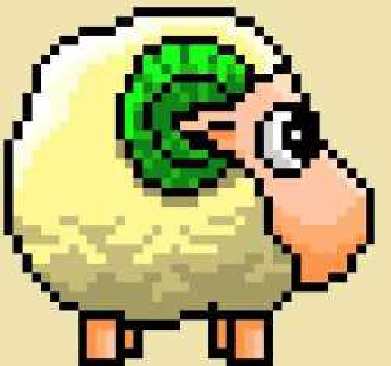
\includegraphics[width=0.75\textwidth]{kuvaesimerkki.pdf}
\caption{Kuvan elementit.}
\label{kuvaesimerkki}
\end{center}
\end{figure}


Kuvien kokoon on kiinnitettävä huomiota. Käytettyjen merkintöjen
on oltava helposti luettavissa ja selkeät. Esimerkiksi
suorituskykykäyriä esitettäessä akselit on nimettävä, asteikot
merkittävä ja käytetyt yksiköt tuotava selkeästi esiin.
Samankaltaisia asioita esitettäessä useammalla kuvalla on
syytä käyttää samaa mittakaavaa vertailun helpottamiseksi.

Kuvan otsikko kirjoitetaan kuvan alle ja sen tulee olla mieluummin lyhyt
ja ytimekäs kuin liian selittelevä.
Samoin toimitaan taulukoiden otsikoinnissa.

Kuvat ja taulukot numeroidaan juoksevasti. Pitkissä teksteissä käytetään
kaksitasoista numerointia (esimerkiksi Kuva 3.1) pääluvuittain, lyhyissä
riittää yksitasoinen numerointi.


Kuva- ja taulukko-otsikoiden yhdenmukaiseen esitystyyliin on syytä kiinnittää
huomiota, samoin mm. välimerkkeihin. Luontevaa on käyttää
kuvatekstin lopussa pistettä, ovathan useimmat kuvateksteistä virkkeitä. 

(Kuvien ja taulukoiden otsikointityyli vaihtelee
kustantajittain ja julkaisuittain. Samoin tuntuu suositeltava käytäntö
Tietojenkäsittelytieteen laitoksen sisällä vaihtelevan taulukon
otsikon sijainnin suhteen.)


\section{Otsikot}

Otsikoissa voi käyttää muusta tekstistä poikkeavaa kirjasintyyppiä,
alleviivausta, suurempaa kirjasinkokoa tms.\ erotuskeinoa, yleensä
kuitenkin vain yhtä näistä, koska kovin monta erilaista kirjasintyyppiä
ja -kokoa tekee ulkoasusta helposti sekavan.  Otsikoiden esitystavan on
oltava johdonmukainen läpi koko kirjoituksen. Numeroimattomia
''ylimääräisiä'' otsikoita ei tule yleensä käyttää.


\section{Mallin käyttö}

Voit käyttää tätä kirjoitusta mallina oman opinnäytteesi ulkoasua
varten. Eri tekstinkäsittelyjärjestelmissä käytössä olevat yksityiskohdat kuten
kirjasintyypit ja -koot ja rivivälit  poikkeavat toisistaan, joten
pienet poikkeamat ovat toki hyväksyttäviä.

Tieteellisen kirjoittamisen kurssin luennoilla ja
liitteenä olevassa ohjeessa annetut töiden ohjeelliset sivumäärät
koskevat työtä, joka vastaa ulkoasultaan tätä ohjetta (kirjasinkoko
12~pistettä). Tässä tekstissä keskimääräinen rivin pituus lienee noin
80~merkkiä ja sivun pituus 35-40~riviä.
Sivumääriin lasketaan varsinaisen tekstiosuuden pituus ja lähdeluettelo
(arabialaisin numeroin numeroitu osuus), ei kansilehteä, tiivistelmää
eikä sisällysluetteloa. Sivumääräarviossa otetaan huomioon hyvin vajaat
sivut, joita syntyy paljon lyhyiden lukujen ja taittotyyliin määritellyn
luvun avauksen pakottaminen oikeanpuolimmaiselle sivulle. 

\chapter{Yhteenveto}

Tämän kirjoituksen tarkoituksena on toimia muistilistana eräistä
esitystavallisista säännöistä, joihin harjoitusten ja tutkielmien
kohdalla on syytä kiinnittää huomiota.

Annetut ohjeet on laitoksen henkilökunta muotoillut yhdessä keskustellen
ja noudattaen oman tieteenalansa perinteitä. Eri erikoistumisaloilla ja
erilaisillaa määräävässä asemassa olevissa julkaisufooruilla käytänteet
vaihtelevat ja nuorten tutkijoiden onkin tiedostettava ero yleisten
sisältöohjeiden ja teknisten muotoilusääntöjen välillä. Aina tekstin
valmistuessa on tarkastettava erikseen, täyttääkö se annetut
pituusrajoitteet ja vastaako se annettuja muotoiluohjeita, olivatpa ne
kuinka pikkutarkkoja tahansa. Tarkasta sääntöjen noudattamisesta syntyy
yhteinäisyyttä kokoovan julkaisun tasolla, mikä helpottaa lukijoiden
työskentelyä.

Tämä ohje vastaa vain asettelullisiin kysymyksiin ja sen rinnalla on
syytä tutustua materiaaliin ja luentoihin, joissa keskitytään tekstin
varsinaiseen sisältöön. Olennaisin väline on kuitenkin akateemisesti
pidemmälle ehtineen, jo julkaisuja rakentaneen ohjaajan palaute ja
mentorointi.


%%
\chapter{Introduction}


In all writing for publication, the writer's freedom of creation and expression are limited by a number of guidelines and specific regulations.

At best, a familiar set of regulations shared by reader and writer can create a kind of support network that allows the message to be relayed without distortion. It will be easier for readers to find 
the pertinent contents in a piece of writing if its layout and structure are the same as they are used to. This also applies to writers. When writers follow a set presentation model, 
they do not have to waste time on considerations that are secondary to the work itself, but they can concentrate on polishing the contents of the text. This means that it is a good 
idea to practice following the rules for the layout, though you may think you know how to select a better way to present your work.

This is a guide for the layout and structure of theses and essays at the Department of Computer Science at the University of Helsinki. It is thus applicable to the course 
Scientific Writing, the software engineering projects, seminars, and MSc theses. (This is an updated version of 
the previous guide written by the course lecturers \citep{erkio01, erkiomakela96, erkio94, verkamo92}.)

The \LaTeX\ guide and \LaTeX\ style that has been  published on the department's web site can be used as support for this guide.


\chapter{Structure}

Let us start by looking at the sections expected to be in a scientific text. Keep in mind that the same expectations go for all kinds of technical writing.
However, this document in itself, is not a scientific or a research
text, so there will be content lacks in terms of research question
setting in the introduction and evaluative material in the last sections.

\section{Abstract or summary}
%\enlargethispage{5mm}


The summary page contains the following elements: the bibliographical data of the work, an abstract, topic classification, 
and the key words. The bibliographical data consists of title, name of the author, place of publication, date of publication, and number of pages.

The abstract should be short, generally one paragraph (100 words maximum) explaining the main contents of the work: topic, methodology and results.


 Topics are classified according to the ACM Computing Classification System
(CCS). A small set of paths (1-3) should be used, starting from any top nodes
referred to bu the root term CCS leading to the leaf nodes. The elements
in the path are separated by right arrow, and emphasis of each element individually can be indicated
by the use of bold face for high importance or italics for intermediate
level. The combination of individual boldface terms may give the reader
additional insight. 

\section{Introduction}


The purpose of the introduction is to introduce the goals of the work in general terms. Describe topic, 
methodology and results (as in the abstract, but expand it).
In order to provide the reader a good starting point for
interpretations, it is good to start the introduction by
contextualisation of the challenges and solutions to be discussed. For
example, why a certain domain has a particular challenge and who are
intended to benefit from the solutions proposed.

The length of the introduction depends on the length of the whole work. A few pages of text does not need a 
separate introduction, since it is an expanded summary in itself. The introduction to a 10-page text can 
be 1--1.5 pages long. For a 50--70-page MSc thesis, a 2--4-page introduction seems reasonable.

The introduction should shortly describe the problem field of the whole work, the plot, and the conclusions, 
in general terms. After reading it, the reader may decide whether to go deeper into the topic by reading the whole text.


\section{Topic chapters}

The nature of the matter at hand determines how the topic chapters are disposed.
In order to guide the reader, it is a good idea to start each main chapter with a short paragraph 
on what the main topic of the chapter is and how it progresses from one sub-chapter to the
next. Especially relevant is to express how concepts, challenges,
solutions and research steps are bound together. There should be enough
guidance for the reader to allow expectation of the right storyline.


Basic rule for easy to follow text is to use the natural emphasis of the
text structure to support the content matter key concepts and thought
processes. This means using openings of sectiosn and text paragraphs for
key arguments and information moves, while the internal parts of
paragraps are filled with supporting aspects that those less familiar
with the topic area need. Those with better background knoweldge can
quickly skim trhough the text without loosing any essential arguments.

Each author has his or her personal ryhtm in the text, which is visible
for the reader as the length of text paragraphs and complexity of
thought chains within. A good policy is to take only one information
move or transition per paragraph. This way the text stays easy to follow.

Signs of problems with the disposition of the text are easily seen in texts
with only one sub-chapter, or with more than two chapter levels (main and sub-chapters). There may be justifiable reasons to use three-level 
headings in some technical documents. Single sentence text paragraphs
are also to be avoided.



%\pagebreak
\section{Reference usage}


Relevant learning targets include superficial knowledge of several
citation styles and capability (and willingness) to follow a given
style and ordering of entires and bibliographical details in the list of references.
These aspects are essential as the approval of a PhD manuscript or
journal article may depend on them.

Disregard of which style you use, 
references are always placed inside sentences.  This means that e.g. a separate reference at the end of a paragraph would be inappropriate.

The structure of the text must clearly show what the reference relates to.  At the same time, it 
shows how long a piece of the text that the reference relates to.

Efficient positions for citations are right after the introduction
(definition) of a concept, a methods or such, or in the end of a claim
from the reference material. Furthermore, if quoting verbatime one must
use citation marks.

The text structures and wordings, in addition to the location of
ciations must clearly express whether claims or arguments are 
authors' own, or if they come from the contribution of others. Thus is
is of bad style to open a section by listing the citations on which the
section is based on. Such method can further indicate more serious
problems like following reference material as it is instead of analysing
and synthetising material into new though processes. 


\section{Conclusion}

At its simplest, a conclusion is merely a weak revision of the main points of the text.  All more valuable 
conclusion sections contain comments on e.g. the value of results, how the work relates to its environment, or 
future visions. This kind of evaluations should be well-grounded in fact, though, or the conclusion 
might inadvertently seem comical. 

\section{Creating the list of references}

The following guidelines should be followed when creating lists of reference for the 
assignments during the course Scientific Writing.

The guidelines are backed by two main goals: to make it as easy as possible to find the 
referenced source, and to show what kind of evaluation process the referenced work has undergone. For these reasons
\begin{itemize}

\item the reference notes should always be so exact that the source can be recognized and found in catalogues and libraries

\item different types of sources (monographs, conferences, journals) have to be easy to distinguish from each other, and 

\item the different parts of the list must conform to each other, especially for each source type.
\end{itemize}


Independent of the citation style in use, 
the sources are listed alphabetically according to the author's name, and works by the same 
author (group of authors) in the order in which they have been published. If some publication 
does not have an individual writer, it is alphabetized according to its name.


The following information should be given on each source independent of
the citation style:
\begin{itemize}
\item
Name(s) of author(s) (surname, initial letters of first names) in the original order; if there are more 
than three authors, we can write the name of the first author and {\em et al.} instead of the other names.

\item
the name of the publication or article in its original form

\item
place of publication:

\begin{itemize}

\item
of monographs: publisher, place of publication (can be omitted if the publisher is well known), year
\item
of journal articles: name of journal, volume, issue, year and month (in parenthesis)

\item
of articles from article collections (such as conference publications):
\begin{itemize}

\item name of collection, editor, publisher, place of publication and year 

{\em or}

\item conference name, coordinator, place and time,

\end{itemize}

\item
of a report: series, report number, place, publisher and year

\item
of a web source: URL, validity date, possibly the date when referenced in square brackets

\end{itemize}

\item
page numbers, if the source is an article or constitutes a chapter in a compilation.
\end{itemize}


When using web sources, you should keep in mind that the threshold for publication on the web 
is non-existent. It is better to concentrate on the publications of well-known scientific 
publishers and the technical standards for which the web is the only publication channel. If 
the same publication is available on paper, refer to that primarily and add the URL as a complement.


The list of references gives an example of a text that has been published through many 
channels~\citep{abiteboul,dietinger}and another example that shows a standard that has 
been disseminated only through the web~\citep{bray}. For web-based
references it is important to give both the publication date and the
time of reading and interpreting the material. The content is prone to
change, and dating your use, you protect your interpretations for
unnecessary accusations of being faulty, if it is known which version
you used.



The list of references for a text should list exactly the sources that the text refers to. 
The list of references for this text is an example of how to present sources, 
which is why it contains ''extra'' sources.


In any style,
put a full stop after the name of a publication or article, as well as after the bibliographical 
data of each reference. Separate the other pieces of information with a comma. As is normal in 
Finnish, only the first letter of the first word in the heading is capitalized, but in the titles of 
conferences and compilations, each major word is capitalized (not articles or prepositions). See the 
appended example for a model. For the sake of clarity, it is best to write {\em In the work} before 
the name of a compilation, except in the case of conference publications where the name starts with 
the abbreviation {\em Proc.} (for Proceedings). In such cases, no complement is necessary. You can 
see the difference by comparing the layouts of the references ~''\citep{dantowsley90}'' and~''\citep{gannonetal89}'' .
In case of other citation styles, it is likely that you can trust the
results given by the automated reference management tools.

\chapter{Layout}

This chapter discusses the main issues of the technical presentation of a text.


\section{Disposition of text sections}


Each text should include a separate cover page, as in this model. The second page contains an 
abstract, followed by a table of contents (on one or more pages), and then the main text.  
Pagination starts on the first page of the main text (with the Arabic numeral 1). (Rigorous writers 
leave out the number from the first page.) All the (numbered) headings and their page numbers should be 
written into the table of contents. Many word-processing systems create the table of contents automatically 
so that the writer does not have to worry about updating page numbers as the work progresses. If writers 
wish to, they can paginate the table of contents and previous pages separately (with Roman numerals), e.g. like this model.

After the main text, but as part of the text body, comes the list of references; its heading is 
not numbered. Any possible appendices are added after the list of references, with headings and internal page numbers.

%\enlargethispage{5mm}

If you want to make a coherent list of figures, algorithms and tables, this list should be placed i
mmediately after the table of contents. The value of such lists is a matter of opinion, so there 
is no need to create one --- especially if your word-processing software does not support it --- unless your instructor explicitly asks for it.

If for some special reason you want to add an alphabetical index top your work, it should be placed after 
the list of references and before appendices. An index should be noted in the table of contents, as s
hould the list of references (unnumbered chapter). Writers who want to create an index should use the automatic support their word-processing system offes.

\section{General text layout}

Nowadays you may plan your text to be printed on single side or double
side, with line spacing one, for the final copy.

For reviewing and feedback purposes, check with your readers for their
preferences. Most read and comment on paper and need some space for
marking. 
For drafts you can use wide margins too. 
Both margins should also be fairly broad (ca.~3~cm): the wider left margin is needed for binding the text and the
right one for the instructor's comments.  Leave enough space (2--3~cm) at the top and bottom, as well.

The most effective way to distinguish features like chapters, figures, etc,  is to have enough space 
in your text.  Separate paragraphs from each other with one and chapters with a few empty lines.  If a 
new chapter is about to start at the bottom of a page (with only one or two lines of text), it is better 
to start it on the next page.  However, it is not necessary to start every chapter on a new page, especially 
not with a short text; if the text contains many pages that are nearly empty, readers might suspect that the 
writer has tried to make it look longer than it is.


Any empty space may be utilized for displaying figures and tables.  Especially if a text is written with the 
same type of text throughout, empty lines are necessary for separating e.g.~text from tables.  Empty space 
is cheap, but adds to the clarity and readability of a text.

\section{Figures and tables}

%\enlargethispage{5mm}

All figures and tables should be placed as near the (first) place in the text that refers to them, but 
not before this reference. The text should also explain what the writer wants to illustrate with the 
figure. Figures can be interpreted in many different ways, so the reader needs guiding.

Figures should never be placed immediately under the heading of a chapter, but chapters should always 
start with text. Figures should not be placed in the middle of a paragraph (much less a sentence), except 
if the figure is placed at the top or bottom of a page and it is clear that the paragraph continues.

Figures do not always have to be placed immediately after the paragraph that refers to them. If there is 
not enough space for a figure on the same page as the paragraph that refers to it, the rest of the page 
should not remain empty, Though the figure is inserted on the following page. However, the figure should 
never be more than one page away from the reference.


The image~\ref{kuvaesimerkki} shows how to present a figure. You must pay attention to the visibility of 
figure parts and text, to the numbering of figures, and captions. 

\begin{figure}[ht]
%\begin{figure}[tbh] t= top, b = bottom, h=here
\ \newline
\begin{center}
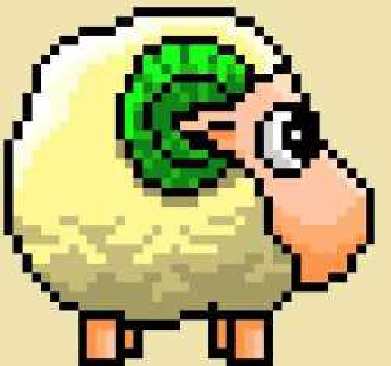
\includegraphics[width=0.9\textwidth]{kuvaesimerkki.pdf}
%\rotatebox{90}{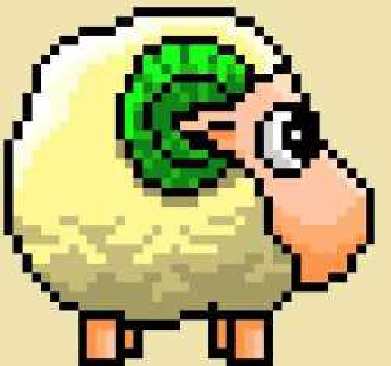
\includegraphics[scale=.75]{kuvaesimerkki.pdf}}
\caption{Figure elements.}
\label{kuvaesimerkki}
\end{center}
\end{figure}


We must also pay attention to the size of figures. Any annotations must be clear and easy to read When 
presenting performance curves, for example, the axels have to be named, the scale notated, and the units 
clearly presented. If you present many things with similar figures, you should use the same scale for easy comparison.

The caption of a figure should be written underneath it, and it is preferable that it be short and to 
the point than too explicit. The same goes for table captions.

Figures and tables should be numbered progressively. In long texts, two-level numbering should be 
used (e.g. Figure 3.1) according to the chapter number, but in shorter texts, one-level numbering is good enough.


You should pay attention to presenting figure and table captions consistently, as well as to punctuation 
marks. It is natural to put a full stop after a caption, since they are most often full sentences. 

(The style for figure and table captions vary according to publisher and publication. The recommendations 
at the Department of Computer Science also seems to vary with respect to where the caption should be placed.)


\section{Headings}

You can use a different font in headings than in the rest of the text, or underlining, larger fonts, or other 
methods of emphasis, but generally it is preferred that you only use one of these methods, because if there are 
very many font types and sizes, the layout looks messy.  The format of headings must be consistent throughout 
the text. You should not use any unnumbered ''extra'' headings.


\section{Using this model}

You can use this text as a model for the layout of your own assignment. The font types and sizes, 
line spacing, etc vary according to word-processing system, so small deviations from the rule are acceptable.

The directive number of pages for written assignments given during the lectures for the Scientific-writing 
course and in this guide are applicable to assignments with a layout like this guide's (font size 12 points). The 
average line in this text should consist of about 80~characters and one page about 30~lines. The number of pages 
includes the text itself and the list of references (the part paginated with Arabic numbers), not the 
cover page, summary, or table of contents.

\chapter{Conclusion}

This text is a checklist for some of the rules governing written presentations, which you should 
keep in mind when writing exercises and theses.

This collection of advise has been compiled by staff members as the
result of discussions on general good writing habbits in computer
science. The consensus is that all young researchers and academic degree
holders must be able to seek and follow instructions of layout and
structuring of texts depending on the contribution they are working on. 
This set of instructions aims at unifying the looks of theses and other
study reports from the department, but it is also a representative of
the instruction sets students will meet later.

This set of instructions only address the looks of the document. Other
instructions must be sought, read and gained experience with in order to
learn to select the suitable semantical contents for the scientific texts.



\end{appendices}
%%%%%%%%%%%%%%%%%%%%%%%%%%%%%%%%%%%%%%%%%%%%%%%%%%%%%%%%%

\end{document}
